\documentclass[a4paper,11pt,oneside,%twoside to print on the back of pages
headsepline,												% Linie für Kopfzeile
footsepline,												% Linie für Fußzeile
bibtotocnumbered									% numb point literaturverz in inhaltsverz => bibliography=tot ocnumbered
]{scrreprt}
%----------------------------------------------------------------------------------------------------------------------------------------------
% STANDART LIBS
\usepackage[T1]{fontenc}
\usepackage[utf8]{inputenc}
\usepackage[ngerman]{babel}    % Deutsche Sprache in automatisch generiertem

% DRUCKBEREICH: \areaset[BCOR]{textwidth}{textheight} %TODO understand
% BCOR ist "Binding Correction", also wieviel Innenrand verloren geht
% A4 hat 297mm x 210mm
% wenn keine Marginalien, dann ist Breite 15cm vielleicht besser
\areaset[1.5cm]{14cm}{25cm} 
%% Die folgende Zeile sorgt dafür, daß die Fußnoten eingerückt werden,
%% und zwar um 2em (class scrbook).
\deffootnote{2em}{2em}{\textsuperscript{\normalfont\thefootnotemark} }

%----------------------------------------------------------------------------------------------------------------------------------------------
% ADDITIONAL LIBS

\usepackage{grffile} %remove file names of images

% Wrapping text around figures
\usepackage{wrapfig}  %
% containers for things that cannot be broken over a page -> example table, figure
\usepackage{float}
% provides many ways to customise the captions in floating environments
\usepackage{caption} % http://www.ctex.org/documents/packages/float/caption.pdf
% same for subfigues
\usepackage{subcaption} % hint include subpicture

%% Unterstützung für Graphiken und Farben
\usepackage[pdftex]{graphicx}
%\usepackage[pdftex]{color}
%\definecolor{DSblue}{rgb}{0,0,0.9}   % example defining a color



% INDEX/GLOSSARY %TODO
%Defines commands for use with MakeIndex
%\usepackage{makeidx} % -> en.wikibooks.org/wiki/LaTeX/Indexing pctex.com/files/managed/3/3a/makeindx.pdf
%\usepackage[xindy,toc]{glossaries}
\usepackage{acronym} %Abkürzungsverzeichniss

%BIBTEX
%used by biblatex for qutes
\usepackage[babel,german=quotes]{csquotes} % load after inputenc
% cite package -> 1. pdflatex xx.tex 2. biber xx 3. pdflatex xx.tex
\usepackage[style=authoryear,backend=biber]{biblatex} %TODO check diff cite styles
% loads the bib file
\addbibresource{bachelorBib.bib}


% cross referencing and hyperrefs
\usepackage[                % FIXME explain
   pdftex,                  % Ausgabe-Medium: PDF
   colorlinks=true,         % farbige Links in der Bildschirm-Version?
   pdfstartview=Fit,       % wie soll Acrobat starten?
   linkcolor=black,         % Farbe für Querverweise
   citecolor=black,         % Farbe für Zitierungen
   urlcolor=black,          % Farbe für Links
   bookmarks=true
   ]{hyperref}
% non clickable URL   		
\usepackage{url} %TODO remove if hyperref is better

% TODONOTES -> http://tex.stackexchange.com/questions/9796/how-to-add-todo-notes
\usepackage{lipsum}                     % Dummytext
\usepackage{xargs}                      % Use more than one optional parameter in a new commands
\usepackage[pdftex,dvipsnames]{xcolor}  % Coloured text etc.
% -> www.tex.ac.uk/ctan/macros/latex/contrib/todonotes/todonotes.pdf
\usepackage[colorinlistoftodos,prependcaption,textsize=tiny]{todonotes}
\newcommandx{\unsure}[2][1=]{\todo[linecolor=red,backgroundcolor=red!25,bordercolor=red,#1]{#2}}
\newcommandx{\change}[2][1=]{\todo[linecolor=blue,backgroundcolor=blue!25,bordercolor=blue,#1]{#2}}
\newcommandx{\info}[2][1=]{\todo[linecolor=OliveGreen,backgroundcolor=OliveGreen!25,bordercolor=OliveGreen,#1]{#2}}
\newcommandx{\improvement}[2][1=]{\todo[linecolor=Plum,backgroundcolor=Plum!25,bordercolor=Plum,#1]{#2}}
\newcommandx{\thiswillnotshow}[2][1=]{\todo[disable,#1]{#2}}

% Print graphics
% tikz print graphs: http://www.texample.net/tikz/examples/
% bytefield – Create illustrations for network protocol specifications

% source code include
\usepackage{listings} % -> %TODO use minted
\usepackage{minted}

\makeatletter
\newcommand*{\rom}[1]{\expandafter\@slowromancap\romannumeral #1@}
\makeatother

%----------------------------------------------------------------------------------------------------------------------------------------------
% ADDITIONAL LIBS TO CHECK

%linien in Tabellen
\usepackage{booktabs}
\usepackage{anysize}
\usepackage[onehalfspacing]{setspace}


% math for matrix and $$
%\usepackage{amsmath}
%\usepackage{amssymb}

%\usepackage{lmodern}

%\usepackage{multido}    % FIXME ???????????
%\usepackage{everysel}   % FIXME ???????????
 
%% besserer Flattersatz: \RaggedRight
\usepackage{ragged2e}

% from exposee
\usepackage{latexsym}         % Fuer recht seltene Zeichen

\usepackage[a4paper,lmargin={2.5cm},rmargin={2.5cm},tmargin={3cm},bmargin={2.5cm}]{geometry}
\usepackage{enumerate}

\newcommand{\HRule}{\rule{\linewidth}{0.5mm}}

\pdfinfo{
	/Title		(Synchronisation von Binärbaum-indexierten, verteilten InMemory-NoSQL-Datenbanken)
	/Subject		(Bachelorarbeit)
	/Author		(Paul Kitt)
}
%----------------------------------------------------------------------------------------------------------------------------------------------
\pagenumbering{roman}
\begin{document}

%TODO set 1,5 zeilenabstand , verdana, schriftgroesse 10
%TODO check bewilligten title 


\begin{titlepage}
	\begin{center}
		\begin{figure}[!htb]
			\minipage{0.5\textwidth}
				\begin{center}
			  		
\includegraphics[width=0.5\textwidth]{bilder/htwLogo.jpeg}
				\end{center}
			\endminipage\hfill
		 	\minipage{0.5\textwidth}
				\begin{center}
			 		
\includegraphics[width=0.5\textwidth]{bilder/Spinning_O_Wheel-200.png}
				\end{center}	
			\endminipage
		\end{figure}
	
		 \vfill
		 \HRule \\[0.4cm]
	    {\bfseries\Large
	        \begin{LARGE}
	        Synchronisation von Binärbaum-indexierten, verteilten
			InMemory-NoSQL-Datenbanken\\
	        \end{LARGE} 
	    }    
		\HRule \\[1.5cm]
			\begin{minipage}{1.0\textwidth}
				\begin{flushleft}
				\Large	Abschlussarbeit
				\end{flushleft}
			\end{minipage}
			\vfill
			\begin{minipage}{1.0\textwidth}
				\begin{flushleft}
					\Large zur Erlangung des akademischen Grades\\
					\Large Bachelor of Science (B.Sc.)
				\end{flushleft}
			\end{minipage}
			\vfill
			\begin{minipage}{1.0\textwidth}
				\begin{flushleft}
					\Large an der
				\end{flushleft}
			\end{minipage}
			\vfill
			\begin{minipage}{1.0\textwidth}
				\begin{flushleft}
					\Large Hochschule für Technik und Wirtschaft Berlin\\
					\Large Fachbereich Wirtschaftswissenschaften \rom{2}\\
					\Large Studiengang Angewandte Informatik\\
				\end{flushleft}
			\end{minipage}
			\vfill
			\begin{minipage}{1.0\textwidth}
				\begin{flushleft}
					\Large 1. Prüfer: Prof. Dr.-Ing. Hendrik Gärtner\\
					\Large 2. Prüfer: Diplom Informatiker Jens-Peter Haack\\ 
				\end{flushleft}
			\end{minipage}
			\vfill
			\begin{minipage}{1.0\textwidth}
				\begin{flushleft}
					\Large Eingereicht von Paul Kitt
				\end{flushleft}
			\end{minipage}

		\vfill
		\begin{minipage}{1.0\textwidth}
			\begin{flushleft}
				{\Large \today}
			\end{flushleft}
		\end{minipage}
		\vfill

	\end{center}
\end{titlepage}
\tableofcontents

	%---------------------------------------------------------------------------------------------------------------------------------------------------	
\chapter{Einleitung}
\pagenumbering{arabic}
\todo[inline]{Hintergrund, größerer Rahmen, kurze Aufgabenstellung}
 		\begin{enumerate}[1.]
			\item  Problemstellung und Motivation
			\item Zielsetzung
			\item Rahmen und Aufbau der Arbeit
		\end{enumerate}
		
	Mögliche Punkte:
	-> Motivation
	-> Aufgabenbeschreibung
	-> Inhalt und Aufbau der Arbeit	
		
	%---------------------------------------------------------------------------------------------------------------------------------------------------	
\chapter{Grundlagen}

In dem Kapitel Grundlagen wird auf die theoretischen Bestandteile und Konzepte dieser Arbeit eingegangen. Dabei werden diese näher erläutert und ihre Funktionsweise erklärt.
Zunächst wird der \enquote{elastische Binärbäum} betrachtet, welcher Grundlegend zur Indexierung von Daten in dieser Arbeit dient. Anschließend wird auf das Datenbankformat NoSQL und auf damit zusammenhängende Konzepte wie das CAP-Theorem, eingegangen. Zum Schluss dieses Kapitels werden zwei Replikationsstrategien, die in verteilten System zum Einsatz, erklärt.   

\section{Elastische Binärbäume}
\label{sec:ebTreeGrundlagen}
Bei den \enquote{elastischen Binärbäumen}, weiter als \enquote{EB-Bäume} abgekürzt, handelt es sich um eine speziell optimierte Variante des \enquote{Binären Suchbaumes}. Binärbäume zeichnen sich dadurch aus das sie der Ordnung zwei entsprechen. Dies Bedeutet das Knoten maximal zwei Kinder, welche mit links/0 und rechts/1 adressiert werde, besitzen kann \autocite[251]{Ottmann2002}.
 Entwickelt wurden das Konzept von Willy Tarreau \autocite{Tarreau} im Rahmen einer Forschung zum Thema \enquote{Event-scheduling for user-space network applications}. Es eignet sich speziell für Betriebssystem-Scheduler, bei welchen schnelles Priorisieren nach Zeit oder Dringlichkeit wichtig ist. Daten die mit Binär- oder Ganzahlen, wie Integer oder Long, indexiert werden, können in dieser wenig bekannten Datenstruktur sehr effizient verwaltet werden. Dabei ist der \enquote{EB-Baum} sehr performant wenn es zu sehr vielen den Baum verändernden Operationen kommt wie e.g. dem Einfügen, dem Ändern, das Abfragen oder Löschen  von Datensätzen kommt\autocite{Tarreau}.
Einfügeoperationen und das Abfragen von Blättern wird in O(log n) bewältigt. Löschen in O(1).\\

Als Ausgangskonzepte seiner Entwicklung dient der \enquote{balancierte Binärbaum} und der \enquote{Radixbaum}. Bei einem \enquote{balancierten Binärbaum} haben  Operationen wie Löschen von Blättern  eine Komplexität von O(log n). Das gesuchte Speicherkonzept aber soll gerade Operationen wie diese möglichst schnell bewältigen. Dieser signifikante Nachteil des \enquote{balancierten Binärbaumes}, soll mit der Entwicklung von Tarreau ausgeglichen werden. Bei den \enquote{Radixbäumen}, die sich laut dem Entwickler Willy Tarreau\autocite[Absatz Introduction]{Tarreau} im Bezug auf Geschwindigkeit sehr gut eigenen, wird aber im Betrieb das allokieren von Speicher und die damit verbundene \enquote{Garbage Collection} zum Perfomanceproblem.\\

Daher ist der \enquote{EB-Baum} eine hybride Form aus Beiden um diese Mängel auszugleichen. Er ist nicht balanciert was in besonderen Fällen zu einer schlechteren Leistung, als die eines \enquote{balancierten Binärbaumes}, führt. Die Blätter des Baumes sind von links nach rechts aufsteigend, nach einem Sie adressierendem Schlüssel, sortiert.
Eine weitere Besonderheit des \enquote{EB-Baum} ist, dass seine maximale Höhe durch den Datentyp der Schlüssel bestimmt wird. So kann Beispielsweise ein Baum der den Datentypen \enquote{Long} für seine Schlüssel verwendet maximal 64 Ebenen besitzen, da der Datentyp aus 64 Bit besteht. Der Schlüssel adressiert ein Blatt durch die Abfolge der Bits in seiner binären Repräsentation und dient wie eine Art binäre Karte. Falls ein Blatt lokalisiert werden soll, wird der Baum von der Wurzel aus Knoten für Knoten durchlaufen. Das für den Knoten repräsentative Bit des Schlüssels gibt dabei den Weg vor.

\subsection{Besonderheiten des Baumes}
Durch die besondere Beschaffenheit des Baumes lassen sich viele Operationen sehr leicht umsetzen wie:
\begin{itemize}
	\item \textbf{Abfragen}
	\begin{itemize}
		\item des kleinsten und größten Schlüssels
		\item des nächst kleineren oder größeren Schlüssels zu einem gegeben Schlüssel
		\item und genaues lokalisieren eine Schlüssels
		\item des nächst kleineren Schlüssels falls der Gesuchte nicht enthalten ist
		\item von Bereichen durch ein Prefix
		\item des vorherigen oder nächsten unterschiedlichen Schlüssels zu einem gegeben Schlüssel
	\end{itemize}
	\item \textbf{Einfügen}
	\begin{itemize}
		\item vom gleichen Schlüsseln und deren Speicherung(Falls ein Schlüssel bereits existiert wird ein Duplikat angelegt)
		\item von nur einzigartigen Schlüsseln(Falls der Schlüssel vorhanden ist, wird der  Existierende Schlüssel zurückgegeben)
	\end{itemize}
\end{itemize}


\subsection{Aufbau des Baumes}
In dem originalen von Willy Tarreau verfassten Konzept\autocite[Absatz Definitions]{Tarreau} werden die Daten, die der \enquote{EB-Baum} hält, in \enquote{EB Knoten}
gespeichert. Ein \enquote{EB Knoten} bestehen aus zwei Teilen:
\begin{itemize}
\item Knoten: verknüpft Blätter sowie andere Knoten
\item Blatt: ist durch einen Schlüssel adressiert, hält Daten e.g. Referenz auf ein Datenobjekt
\end{itemize}


\begin{figure}[h!]
  \begin{center}
    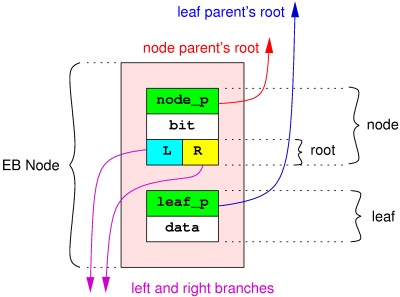
\includegraphics[width=.5\linewidth]{bilder/Ebnode.png}
  \end{center}
 \caption{EB-Knotenelement Ansatz von \autocite{Tarreau}}
\end{figure}
Die Aufgabe eines Blattes ist sehr simpel. Es dient nur dazu eingefügte Daten zu halten. Dabei ist es mit einem Schlüssel adressiert und besitzt eine Referenz auf seinen Elternknoten, sowie auf seinen EB-Ursprungsknoten.\\

Ein jedes Knotenelement besteht aus einer Referenz auf sein höher liegenden Elternknoten, dem Ebenenbit  und zwei Referenzen auf seine Kinderknoten. 
Als Elternknoten wird der direkt über dem Knoten befindliche Knoten bezeichnet. Das Ebenenbit ist eine Zahl und repräsentiert die Position bis zu der sich alle binären Repräsentation aller unter dem Knoten liegendem Schlüssel gleichen.  Alle unter dem Knoten liegenden Schlüssel haben somit bis zu diesem Bit die gleich Bitfolge. Der dritte Teil des Knotens sind die zwei Referenzen seiner Kinder, die entweder auf weitere Knoten oder/sowie Blättern verweisen. Da es sich um einen binären Baum handelt repräsentiert je Referenz das linke Bit 0 und das rechte Bit 1. Auch wenn Knoten sich später verschieben können diese nie unterhalb des mit ihnen angefügten Blattes, oder in einen anderen Zweig des Baumes gelangen. Es ist Möglich das Konzept des Baumes mit sich gleichenden Schlüsseln zu implementieren. Falls Duplikate einzufügen werden können, wird der dem Duplikat zugehöriger Knoten mit einem negativen Ebenenbit versehen. Eine weitere Besonderheit des Baumes ist, dass die Kinder eines Knoten nie unbelegt sind. Nur der Wurzelknoten des Baumes ist eine Ausnahme. Wenn seine zwei Wurzeln auf \enquote{null} referenzieren, ist der Baum leer. Sobald der Baum befüllt wird wächst dieser an seiner linken/\enquote{0-Wurzel}. Die rechte Wurzel referenziert immer auf \enquote{null}. Dadurch lässt sich der der Wurzelknoten einfach erkennen.
Sein Ebenenbit ist die höchste Ebene des Baumes und daher automatisch die Größe des Schlüsseldatentypes, e.g. bei Schlüsseln des Datentypes Long ist das Ebenenbit 64.\\


\section{NoSQL-Datenbanken}
Die Idee der NoSQL-Datenbanken ist anders als mensch erwarten könnte keine neue Erfindung. Schon die 1979 entwickelte \enquote{DBM} beruhte auf einem \enquote{Key/Hash} Konzept und auch in den 80er Jahren waren mit \enquote{Lotus Notes} und \enquote{Berkley DB} bereits Konkurrenz zu den bekannten SQL basierenden Datenbanken existent \autocite[1]{Edlich2010}. Durch die steigenden Anforderungen an moderne Datenbanksysteme kommt es gerade Heute vermehrt zu Entwicklungen von NoSQL-Datenbanken. NoSQL ist nicht durch eine Organisation oder ein Gremium definiert worden sondern viel mehr Sammelbegriff einer neuen Generation von Datenbanken die dann unter dem Titel \enquote{NoSQL} zusammen gefasst wurden. Populäre Vertreter aus dieser Reihe sind e.g. Casandra, Redis, MongoDB. Eine Definition welche Anforderungen eine Datenbank erfüllen muss um in diese Kategorie zu fallen ist daher nicht klar definiert. In \enquote{NoSQL: Einstieg in die Welt nicht relationaler Datenbanken} nähert sich Prof. Stefan Edlich durch folgende Definitionen  einer generellen Beschreibung an. Unter NoSQL wird eine neue Generation von Datenbanksystemen verstanden, die meistens einige der folgenden Punkte berücksichtigen so Edlich\autocite[2]{Edlich2010}:
\begin{itemize}
		\item Das zugrundeliegende Datenmodell ist nicht relational
		\item Die Systeme sind von Anfang an auf eine verteilte und horizontale Skalierbarkeit ausgerichtet
		\item Das System ist Schemafrei oder hat nur schwächere Schemarestriktionen.
		\item Aufgrund der verteilten Architektur unterstützt das System eine einfache Datenreplikation
		\item Das System bietet eine einfache API
		\item Dem System liegt meistens auch ein anderes Konsistenzmodell zugrunde: Eventually Consistent und BASE, aber nicht ACID
\end{itemize}
Die Erweiterung eines bereits festgelegten Datenbankschemas, bei sich veränderten Anforderungen, kann bei relationalen Datenbanken zu Problemen oder zu unerwünschten \enquote{Downtimes} führen. Daher werden Schemarestriktionen gelockert und ein einfaches sowie schnelles, nachträgliches Ändern von Datenstrukturen ermöglicht. Durch Konzepte wie \enquote{Multiversion Cocurrency Control}, kann die Datenstruktur im Hintergrund verändert und sobald der Vorgang abgeschlossen ist als neue Version in Betrieb genommen werden. Sie muss nicht gesperrt werden wie es e.g. einer komplexeren Änderung durch \enquote{ALTER TABLE} und damit verbundenen Anpassungen fordern würden \autocite[3, 40]{Edlich2010}.\\

Das Aufkommen von extrem großen Datenmengen in Bereichen von Terra bis Petabyte sind Heute keine Seltenheit mehr, sondern viel mehr Normalität. Die Entstehung vieler neuer NoSQL-Datenbanken passierte zeitgleich mit der Entwicklung des Web 2.0 und daher sind diese auf das Verwalten sehr großer Datenmengen ausgerichtet.
Dabei spielt die Möglichkeit wie einfach die Datenbank zu skalieren ist eine große Rolle. So müssen diese sowohl vertikal (scale up) als auch horizontal (scale out) Skalierbar sein. Die vertikale Skalierung wird durch ein einfaches Verbessern der Datenbankhardware umgesetzt. Bei der horizontalen Skalierung wird die Masse an Daten und Last auf mehrere Instanzen aufgeteilt und ermöglicht eine kostengünstigere und flexiblere Möglichkeit die Leistung des Systems zu erweitern. Dieser Prozess wird als \enquote{Sharding} bezeichnet.
NoSQL-Datenbanken sind nicht mehr wie viele relationale Datenbanken nur eine Datenbank, sondern von sich aus bereits ein Datenbanksystem oder bieten einfache Möglichkeiten der Erweiterung zu diesem. Die Möglichkeit der Replikation steht dabei an zentraler Stelle, siehe \autoref{sec:VertDB}.\\\\
Je nach Anforderungen orientieren sich die Datenbanken an Modellen wie \enquote{ACID}\footnote{Atomicity, Consistency, Isolation, Durability} oder dem \enquote{CAP-Theorem} und lassen die Restriktionen relationaler Konkurrenten, die sich stark an \enquote{ACID} und dem Konzept der Transaktionen orientieren, hinter sich. So liegen die Ansprüche bei Web 2.0 Anwendungen, wie e.g. Sociale Netzwerke, mehr auf schnellen Antworten, dem Halten immenser Datenmengen und Fehlertoleranz als auf Konsistenz und fehlerfreien Transaktionen.
Nichtsdestotrotz gibt es aber auch NoSQL-Datenbanken die Transaktionen oder  zumindest transaktionsähnliche Prozesse bieten, um auch bereits bekannten Anforderungen zu genügen.

\subsection{Typen}
NoSQL Datenbanken lassen sich in vier Kategorien einteilen:
\begin{description}
   \item[Key/Value Stores] Daten werden in Schlüssel/Werte Paaren gespeichert. Dabei ist es oft möglich die Schlüssel in Namensräume zu sortiert und den Werten Datentypen zu zuweisen. Durch dieses einfache Schema lassen sich die Daten einfach aufteilen. Die Verarbeitung ist ebenso sehr schnell und effizient. Nachteil dabei ist dabei dass nur einfache Abfragemöglichkeiten verfügbar sind \autocite[131]{Edlich2010}.
   \item[Wide Column Stores] Daten werden ähnlich wie bei rel. Datenbanken in Tabellen gespeichert. Werte werden gruppiert und spaltenorientiert in jeweils eine eigene Tabelle geschrieben. Dies ermöglicht ein einfaches Verarbeiten der Daten. Operationen wie Einfügen oder bestimmte Abfragen sind jedoch aufwendig.
   \item[Document Stores] Basieren auf dem Konzept strukturierte Daten in Dokumenten abzulegen. Auf diese wird mittels IDs referenziert und so ein Zusammenhang erstellt. Dateiformate sind dabei: JSON, YAML oder RDF.
   \item[Graphendatenbanken] Eignen sich besonders um den Zusammenhang zwischen Daten abbilden zu können. Die technischen Möglichkeiten immer komplexere Dinge, wie Moleküle oder Linkstrukturen des Internets zu erfassen, steigern den Bedarf diese Daten in einem passendem Schema zu speichern. Die Daten werden dabei in Baum- oder Graphenstrukturen gespeichert.
\end{description}

\section{NoSQL relevante Konzepte}
\subsection{CAP-Theorem}
\label{CAP}
Das CAP-Theorem, auch als Brewer's Theorem bekannt, betrachtet drei Kriterien die an Datenbanken gestellt werden:
\begin{description}
\item[Konsitenz(Consistency)] \enquote{Steht im CAP-Theorem dafür, dass die verteilte Datenbank nach Abschluss einer Transaktion einen konsistenten Zustand erreicht} laut Edlich \autocite[31]{Edlich2010} und Veränderung auf allen Knoten erfolgt sind
\item[Verfügbarkeit(Avaibility)] bedeutet dass jede Anfrage die an einen nicht ausgefallenen Knoten gestellt wird beantwortet wird ganz gleich ob Erfolg oder Fehler \autocite[54]{Fowler2013}.
\item[Ausfalltoleranz(Partition Tolerance)] meint, dass das System im Falle des Ausfalls eines Knoten von Außen betrachtet noch problemlos weiter funktioniert.
\end{description}
Je nach dem für welche Anforderungen die Datenbank ausgelegt ist, erfüllt sie Teile dieser drei Kriterien, aber nie alle drei. 
\subsection{BASE-Konsistenzmodell}
\label{BASE}
Die Abkürzung BASE steht für \enquote{Basically Available, Soft state, Eventual consistency}. Der Ansatz des BASE-Konsistenzmodelles verfolgt eine maximal hohe Verfügbarkeit und Leistung. \enquote{Konsistenz wird dieser untergeordnet. Wo ACID einen pessimistischen Ansatz bei der Konsistenz verfolgt, ist BASE ein optimistischer Ansatz, bei dem Konsistenz als ein Übergangsprozess zu sehen ist und kein fester Zustand nach einer Transaktion} beschreibt Edlich in seinem Buch NoSQL\autocite[33, 34]{Edlich2010}. Der Zustand von Konsistenz wird dabei auch erreicht, aber erst in einem bestimmten Zeitrahmen. Dieser neue Ansatz von Konsistenz wird als: \enquote{Eventually Consistent} bezeichnet. Dabei versteht sich BASE zu ACID nicht als sich gegenseitig ausschließend sondern, laut Eric Brewer \footnote{formulierte das CAP Theorem,Prof. an der UC Berkeley} eher als andere Seite eines Spektrums in dem relationale Datenbanken mehr zu ACID und NoSQL eher zu BASE tendieren.

\section{Verteilte Datenbankarchitekturen und Replikationsstrategien}
\label{sec:VertDB}
Der Schritt von einer einfachen Datenbank zu einem verteilten Datenbanksystem erhöht zwar die Komplexität des Systems, bringt aber je nach Anforderung einige positve Aspekte mit sich. \enquote{Die Replikation ist eine Technik zur Verbesserung von Diensten. Die Motivationen für die Replikation sind, die Leistung eines Dienstes zu verbessern, seine Verfügbarkeit zu erhöhen, oder ihn fehlertoleranter zu machen} beschreibt Coulouris die positive Effekte von Replikation in Verteilte Systeme \autocite[642]{Coulouris2002}. Ein weiterer wichtiger Aspekt von verteilten Systemen ist Transparenz. Andrew S. Tannenbaum erklärt diese in seinem Werk Verteilte Systeme folgendermaßen: \enquote{Das System ist nach außen transparent. Ein verteiltes System, das in der Lage ist, sich Benutzern und Anwendungen so darzustellen, als sei es nur ein einziges Computersystem, wird als transparent bezeichnet} \autocite[21]{Tannenbaum2008}.

\subsection{Master-Slave Replikation}
Bei diesem Replikationskonzept werden die Daten auf verschiedene Knoten repliziert. In diesem Ansatz ist ein Knoten der \enquote{Master} des Datenbankensystems und die anderen Knoten \enquote{Slaves}. Soll durch einen Client etwas verändert werden nimmt der \enquote{Master} dies entgegen und leitet die Schreiboperation an die \enquote{Slaves} weiter. Diese enthalten somit immer den selben Datenbestand wie der \enquote{Master} und sind ein sogenanntes \enquote{Hot Backup}. Um die Leistungsfähigkeit des Datenbanksystemes zu steigern ist es möglich das \enquote{Slaves} Leseanfragen beantworten und damit die Last dieser Anfragen auf alle Knoten verteilt werden kann. Gerade bei Anwendungen mit wenig Schreib- und vielen Leseoperationen steigert dies die Leistung enorm. Zudem kann das System durch hinzufügen weiter \enquote{Slave-Knoten} einfach horizontal Skaliert werden.\\

Kommt es zu einem Ausfall des \enquote{Master-Knoten} können immer noch Leseoperationen von den \enquote{Slaves} verarbeitet und beantwortet werden. In diesem Fall kann ein \enquote{Slave} zum \enquote{Master} werden und dessen Funktionalitäten übernehmen. Fällt ein \enquote{Slave} aus kann dieser mittels des \enquote{Redo-Log}, in welchem der \enquote{Master} Schreiboperationen protokolliert, wieder auf den aktuellen Stand gebracht werden. Diese Replikationsstrategie wird von den Erweiterungen alter relationaler Datenbanken, wie MySQL-Cluster, als auch von neuen NoSQL Datenbanken wie MongoDB verwendet \autocite[40]{Fowler2013}.

\subsection{Multi-Master Replikation}
In \enquote{Multi-Master Replikationen} sind, im Gegensatz zur \enquote{Master-Slave Replikationen}, alle Knoten gleichrangig. Jeder Knoten kann Schreib- und Leseoperationen verarbeiten. Dieser Ansatz macht das Datenbanksystem enorm Leistungsfähig da die Last aller Operationen gleichmäßig auf alle Knoten verteilt werden kann. Die Leistungsfähigkeit des Datenbanksystems kann sehr einfach horizontal, durch das einfügen weiterer Knoten, wie vertikal, durch das Verbessern der Knoten Hardware, nach oben skaliert werden. Fällt ein Knoten aus mindert dies nur die Leistungsfähigkeit des Systems aber nicht seine Funktionalität an sich. Dieser Gewinn an Leistung geht allerdings mit einem Verlust an Konsistenz einher. Solange jedoch eine Änderung nur wirksam wird wenn die Mehrheit der Knoten die Veränderung erhält kann sicher gestellt werden dass ein inkonsistenter Zustand behoben werden kann\autocite[42]{Fowler2013}.

	%---------------------------------------------------------------------------------------------------------------------------------------------------	
\chapter{Anforderungsanalyse}
Im Kapitel Anforderungsanalyse wird das zugrunde liegende Problem dieser Arbeit im einzelnen analysiert. Da die vom Autor verfasste Arbeit in Zusammenarbeit mit einem IT-Unternehmen entstand werden deshalb zu Beginn die Rahmenbedingungen der Kooperation erläutert. Anschließend wird das Problem von anderen Teilaspekten abgrenzt. Daraufhin werden die Anforderungen des in dieser Arbeit geforderten Lösungsansatzes formuliert und des Weiteren eine klare Zielstellung zu definieren.  
Als letzter Absatz in diesem Kapitel wird eine strukturierte Vorgehensweise erläutert.

\section{Betriebliches Umfeld}
Diese von dem Autor verfasste Arbeit entstand in enger Kooperation mit der neu entstehenden \enquote{SpinningWheel GmbH}. Das hier implementierte und getestete Datenbankteilkonzept ist ein kleiner Bestandteil eines großen Softwareprojektes mit dessen Entwicklung die Firma sich beschäftigt. So wurde der Autor mit Idee und Grundkonzept beauftragt und bei deren Umsetzung von Herrn Jens-Peter Haack und Gernot Sänger bei theoretischen Fragen unterstützt.\\

Die \enquote{SpinningWheel GmbH} befasst sich mit der Entwicklung neuer Softwarelösungen für das Backend von Mobilfunkinfrastruktur. Dabei steht das Verarbeiten und Speichern von Mobilfunksubscriberdaten(Nutzerdaten) durch neue technische Möglichkeiten im Vordergrund.

\section{Thematische Abgrenzung}
Die in dieser Arbeit beschriebenen, umgesetzten und getesteten Programmkomponenten sind ein kleiner Teil eines großen neuen, verteilten Datenbankkonzeptes der \enquote{SpinningWheel GmbH} und beschränken sich auf das im Speicher halten von Daten zur Laufzeit. Des Weiteren sind sie auf Synchronisation zwischen Datenbanken zum Ausgleich verpasster Änderungen beschränkt.\\

Alle weiteren Bestandteile einer Datenbank wie das Persistieren, Verarbeiten oder komplexe Abfragen der gespeicherten Daten sind nicht Teil dieser Arbeit und werden nicht oder nur am Rande behandelt.  

\section{Problemstellung}
Durch die in \autoref{sec:VertDB} beschriebenen Replikationsstrategien können die Anforderungen der meisten aktuellen Anwendungen an Konsistenz und Leistung erfüllt werden. Jedoch stellen einige Bereiche wie e.g. Mobilfunk Anforderungen die mit vielen jetzigen Datenbankkonzepten nur schwer oder gar nicht umsetzbar sind. Gerade im Fall Mobilfunk muss dass Datenbanksystem maximal Performant und Ausfallsicher sein. Dazu kommt dass die Last die das System verarbeiten soll so immenz ist das traditionelle Lösungsansätze versagen. Eine Replikation des Datenbanstandes durch eine \enquote{Master-Slave} Hierarchie ist ausgeschlossen, da es bei diesem Szenario zu einem hohem Aufkommen an Schreiboperationen kommt
, wie e.g. beim Wechsel der Nutzer zwischen Mobilfunkzellen. Für die aufkommende Last an Schreiboperationen muss ein Verteilen der Last möglich sein. Zudem muss das System bei Ausfall eines Knotens diesen sehr schnell kompensieren. Fällt der \enquote{Master-Knoten} aus muss ein \enquote{Slave-Knoten} zum neuen \enquote{Master-Knoten} umfunktioniert werden, was bei den gestellten Maßstäben an Verfügbarkeit inakzeptabel ist.\\

 Aber auch der Ansatz vieler bereits verfügbarer \enquote{Multi-Master} Lösungen hat bei derart hohen Anforderungen Probleme. Ein \enquote{Load Balancing} aller Anfragen ist bei dieser verteilten Architektur einfacher möglich, da alle Knoten im System gleichwertig sind. Fällt ein Knoten aus können alle anderen im System seine Funktionalität ersetzen, wobei lediglich die gesamte Leistung des Systems sich verschlechtert. Das Problem hierbei ist nicht der Ausfall an sich, sondern das Aktualisieren eines ausgefallenen Knoten. Je nach dem wie lange dieser Ausgefallen ist, ist der Unterschied zu den anderen Knoten groß. Lösungsansatz ist bei den meisten Systemen mit \enquote{Master-Slave Replikation} als auch \enquote{Multi-Master Replikation} das anlegen eines \enquote{Redo-Log}. In diesem Log werden alle Änderungen protokolliert. Ein veralteter Knoten kann nun mit Diesem alle Veränderungen nachholen. Im Bereich des Mobilfunks kann es aber vorkommen das in der Zeit in der der Knoten nicht erreichbar war so viele Änderungen passiert sind, dass eine derartige Synchronisation nicht möglich ist. Zudem ist diese Lösung sehr unperformant, da falls ein Wert viele Male geändert wurde alle Änderungen Schritt für Schritt durchlaufen werden statt direkt den aktuellen Wert zu übernehmen. Dieses Problem tritt ebenso ein falls sich die Knoten an verschiedenen geographischen Orten befinden und die Verbindung zwischen ihnen unterbrochen ist. Die getrennten Knoten erhalten weiter Veränderungen von Clients in ihrer Nähe, können sich aber erst wenn die Verbindung wieder vorhanden ist synchronisieren. Ein Ausgleich mittels der \enquote{Redo-Logs}, der getrennten Knoten, gestaltet sich hier noch schwieriger.


\section{Zielstellung}
Um die beschriebenen Probleme herkömmlicher Datenbanksysteme und die besonders hohen Anforderungen an Ausfalltoleranz und Verfügbarkeit, die ein Anwendungsgebiet wie e.g. Mobielfunk stellt, erfüllen zu können, ist die Entwicklung eines genau darauf angepassten verteilten Datenbanksystem sinnvoll. Um die Schwierigkeiten einer Synchronisation mittels \enquote{Redo-Log} zu vermeiden muss das System eine intelligente Synchronisationsmethodik besitzen. Ziel dieser Arbeit ist es einen Synchronisationsalgorithmus zu entwickeln und zu testen der dieser Problematik begegnet. Dabei soll die allgemeine Funktionalität des Algorithmus bewiesen und Leistung unter verschiedenen Szenarios analysiert werden.


\section{Anforderungen: Datenbanksystem}
An das Datenbanksystem werden folgend beschriebe Anforderungen gestellt. Der Fokus des Systems liegt auf maximaler Verfügbarkeit und Ausfalltoleranz. Dafür muss eine effiziente Verteilung der Last aller gestellten Anfragen auf die Knoten des Systems möglich sein. Gestellte Lese- oder Schreiboperation eines Clients müssen in kürzest möglicher Zeit verarbeitet und positiv oder negativ beantwortet werden. Jeder Knoten muss in der Lage sein, im Fall eines Ausfalls, alle Funktion eines Anderen binnen kürzester Zeit zu übernehmen. Laut dem CAP-Theorem, siehe \autoref{CAP} geht diese Gewichtung des Systems mit einem Verlust an Konsistenz einher. Dies ist bis zu einem gewissem Grad akzeptabel solange sicher gestellt ist, dass das System nicht einen gewissen Grad an Inkonsistenz überschreitet und inkonsistente Zustände einzelner Datensätze definitiv zeitnah behoben werden. Dies soll durch den später beschriebenen Synchronisationsalgorithmus, siehe \autoref{sec:eBTreeSynchronisation} möglich sein. Das System entspricht somit tendenziell dem BASE-Konsistenzmodell, siehe \autoref{BASE} und kann als \enquote{Eventually Consistent} bezeichnet werden.\\ 

Im Hinblick auf Geschwindigkeit ist das System in hohem Maße fehlertolerant. Mit auftreten von Fehlern und Ausfall wird in einem derart komplexen System gerechnet. Bei Fehlern im System muss sichergestellt werden dass eine Mehrheit an Knoten die Operation fehlerfrei ausgeführt hat. Treten bei der Minderheit Fehler auf sind diese und damit verbundene Inkonsistenzen tolerierbar. Falls aber bei einer Mehrheit Fehler auftreten muss sichergestellt werden dass die Antwort an den Client negativ ist und  wiederholt werden kann.Eine weitere Anforderungen an das System ist Transparenz. Hierbei sind interne Verteilung und Prozesse nach außen nicht nachvollziehbar. Zudem soll seine Leistung horizontal wie vertikal einfach skalierbar sein. Um des Weiteren eine hohe Leistungsfähigkeit zu gewährleisten soll es möglich sein dass der redundante Datensatz eines Knotens durch \enquote{Sharding} auf mehre Hardwareresourcen aufgeteilt werden kann. Um eine maximale Verfügbarkeit der Daten zu ermöglichen müssen die auf allen Knoten verteilten, durch Sharding partitionierten, Teile des gesamten Datenbestands zur Laufzeit des Systems im Arbeitsspeicher gehalten werden.

\section{Anforderungen: Synchronisation}
Aufgabe des in dieser Arbeit betrachteten Synchronisationsalgorithmus ist es den Grad an Inkonsistenz im verteilten Datenbanksystem so gering wie möglich zu halten und zu gewährleisten dass entstandene Inkonsistenzen mit Sicherheit ausgeglichen werden. Dabei werden folgende Anforderungen an den Algorithmus gestellt. Die Synchronisation ist symmetrisch. Dies Bedeutet dass keine Hierarchie, wie e.g. \enquote{Master-Slave}, zwischen den beteiligten Knoten existiert. Die Synchronisation kann von jedem Knoten initiiert und in jede Richtung erfolgen. Der gesamte Synchronisationsprozess ist zustandslos. Somit kann dieser jederzeit pausiert, neu gestartet als auch wieder aufgenommen werden ohne dass Teile des Prozesses wiederholt werden müssen. Selbst das Auftreten von Fehlern, wie Verlust von Synchronisationsnachrichten, oder Veränderung der Datenbestände soll die Funktionalität und Leistung der Synchronisation nur geringfügig beeinflussen. Neue Differenzen zwischen den Knoten die während des Synchronisationsprozesses auftreten müssen jederzeit berücksichtigt und behandelt werden. Der Algorithmus muss in der Lage sein zu erkennen welche Version eines Datensatzes die Aktuellste ist. Anders als bei der Synchronisation mittels \enquote{Redo-Log}, bei der alle Veränderungen eines Datensatzes der Reihe nach durchlaufen werden, soll nur die neueste verpasste Veränderung nachgeholt werden.\\

Das Senden von Synchronisationsnachrichten, bis zum Austausch eines Datensatzes, soll so wenig Ressourcen des Systems wie möglich belegen. Daher sollen die versandten Synchronisationspakete möglichst klein und der Algorithmus adaptiv sein. Während der Synchronisation soll erkannt werden wie gravierend der Zustand an Inkonsistenz gerade ist. Der Algorithmus soll sich selbständig daran anpassen und seine Leistung steigern. Die Effizienz des Algorithmus darf von der Größe des Datenbestandes nur geringfügig beeinflusst werden. So soll das Ausgleichen weniger Unterschiede bei einem großem Datenbestand nicht wesentlich länger dauern als bei einem verhältnismäßig kleinen Datenbestand. Die Synchronisationsmethodik soll in der Lage sein schnell kleine Unterschiede, als auch in einer längeren Zeitspanne Datenbanken, die sich auf völlig verschiedenen Ständen befinden, auszugleichen. Kommt es während des laufenden Betriebes des Systems zu ein signifikanten Anstieg an Inkonsistenz soll der Synchronisationsalgorithmus dies feststellen und darauf aufmerksam machen. Falls der Algorithmus nicht in der Lage ist einen bestimmten Grad an Konsistenz aufrecht zu erhalten, muss dies ebenfalls erkannt und der Administration mitgeteilt werden.\\


\section{Vorgehen}
-> Eingrenzung auf wenige bestandteile der datenbank(halten uIDs, cID, synchro)
-> Implementierung der Basis Klassen und Funktionalitaeten 
-> Implementierung der Simulations und Evaluations elemente
-> Definieren von Tests und deren Analyse
-> performance
-> Unittests: grobe Funktionstests 
Technisches Umfeld:
(-> Scala mit Akka)






%---------------------------------------------------------------------------------------------------------------------------------------------------
\chapter{Konzept alias Definition/Entwurf}
Zu Beginn wird in diesem Kapitel erörtert wie ein verteiltes System konzeptioniert werden muss um den im letzten Kapitel gestellten Anforderungen zu genügen. Anschließend wird auf das Konzept eingegangen nach dem die Knoten in diesem verteiltem Datenbanksystem aufgebaut sind. Die Systematik des in dieser Arbeit untersuchten Synchronisationsalgorithmus wird danach erklärt und im Anschluss auf den Aufbau des programmierten Datenbankprototypen, sowie der sich darüber befindlichen Simulationsumgebung, eingegangen.

\section{Konzept des verteilten Datenbanksystem}
\label{sec:DBSystemConcept} 
Um die, in der Anforderungsanalyse beschrieben, Kriterien zu erfüllen, ist das Datenbanksystem  in verschiedene, gleichrangige Knoten gegliedert. Die dabei verwendete Replikationsstrategie ist \enquote{Multi-Master}. Diese Aufteilung des Systems  soll einem hohen Anspruch an Ausfallsicherheit gerecht werden, sowie eine horizontale und vertikale Skalierung ermöglichen. Die Daten, die das System persitiert, werden auf allen Knoten redundant abgelegt. Die Anzahl der Knoten bestimmt die Ausfallsicherheit des Systems. So kann mit einer größeren Anzahl an Knoten eine höhere Ausfallsicherheit gewährleistet werden. Jedoch steigen damit gleichzeitig die Kosten und der Aufwand, das System zu betreuen, sowie die Komplexität und die Koordination von systeminternen Abläufen. Die Verwendung separater Hardware-Ressourcen und eine Aufteilung in räumlich getrennte Standorte machen das System zudem tolerant gegenüber Hardwareausfällen und nicht-systeminternen Problemen, wie e.g. ein Ausfall der Stromversorgung. Ein Partitionieren der Daten durch Sharding in kleine Einheiten in den Datenbankknoten wird in dieser Arbeit nicht weiter untersucht, bietet aber eine gute Möglichkeit, das System zu optimieren. Damit ist eine horizontale Skalierung des Datenbanksystems möglich, da diese durch die Unterteilung der Daten in der Knoten einfach auf mehrere Ressourcen verteilt werden können. Durch eine Optimierung der Hardwareressourcen des Knotens, oder ihrer Teile, kann das System zudem auch vertikal nach oben skaliert werden. Die Aufteilung der Daten auf verschiedene Instanzen ermöglicht außerdem ein Verteilen der Last. Ein derartiges \enquote{Load Balancing} kann einfach e.g. durch einen Router auf Netzwerktechnikebene koordiniert werden. Das Datenbanksystem ist nach außen transparent. Das System liefert dementsprechend ein Reihe an extern aufrufbarer Funktionalitäten, wie diese aber durch interne Vorgänge bewältigt werden, bzw. wie der Aufbau des Datenbanksystems konzipiert ist, ist nach außen hin nicht ersichtlich.
\begin{figure}[h!]
        \centering
    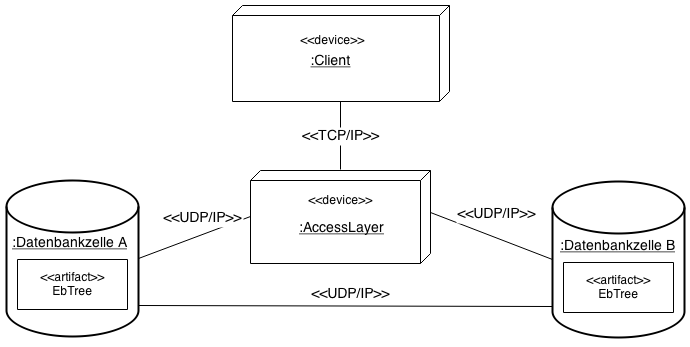
\includegraphics[width=0.9\textwidth]{bilder/uml_deployment_dia.png}
    \caption{UML Deploymentdiagramm des verteilten Datenbanksystems}
\end{figure}
Eine essentielle Komponente in diesem verteilten Datenbanksystem ist die Schnittstelle zu den Clients, der sog. \enquote{Accesslayer}. In diesem werden für neue Daten oder Veränderungen eindeutige IDs erzeugt. Jedem neuen Datensatz wird eine eindeutige Nummer zugewiesen, die ihn adressiert, sowie eine weitere Nummer, die den Datensatz versioniert. Neue IDs steigen mit jeder weiteren Generierung. Wird ein neuer Datensatz eingefügt, oder verändert, sorgt der \enquote{Accesslayer} dafür, dass dieser adressiert, sowie an alle Datenbanknoten gesandt wird. Um eine hohe Verfügbarkeit zu gewährleisten muss der \enquote{Accesslayer} dem Client schnell antworten. Daher innerhalb des verteilten Datenbanksystems Pakete mittels UDP-Protokoll versandt. Antwortet eine Mehrheit der Knoten, in einer festgelegten Zeitspanne, positiv auf die versandte Schreiboperation kann dem Client positiv geantwortet werden. Dabei entstehende Inkonsistenzen werden hin genommen da durch die Synchronisation gewährleistet ist dass diese behoben werden. Um auch hier eine möglichst hohe Ausfallsicherheit und eine Balancierung von Last zu gewährleisten, ist es möglich, dass mehrere \enquote{Accesslayer} parallel arbeiten. Die Koordination der unterschiedlichen \enquote{Accesslayers} ist eine weitere, umfangreiche Aufgabe, die im Rahmen dieser Arbeit nicht weiter erörtert wird.

\section{Konzept des Datenbankknotens}
\label{sec:DBConcept} 

Die grundlegende Idee der oben beschriebenen Datenbank ist, nicht wie in relationalen Datenbanken, Daten durch Tabellen zu gruppieren, sondern die Daten durch viele unterschiedliche Indexe zugänglich zu machen, je nachdem welche Kriterien für eine Gruppierung erforderlich sind. So kann jederzeit durch das Bilden von neuen Indexen auf neue Anforderungen an die Datenbank reagiert werden. Der gesamte Datenbestand des Knotens ist auf Festplatten persistiert, wird aber zur Laufzeit komplett im Arbeitsspeicher gehalten um den Anforderungen an Geschwindigkeit zu genügen. Operationen auf Festplatten verbrauchen, bei den gestellten Anforderungen, zu viel Zeit.\\

Neue Datensätze erhalten bei ihrer zentralen Erzeugung im \enquote{Access Layer} eine eindeutige, aufsteigende ID. Die Nummer ist für alle Kopien innerhalb allen Datenbanken gleich, verändert sich nie und adressiert den Datensatz, bis dieser gelöscht wird. Eine weitere Nummer, die \enquote{Change ID}, symbolisiert den Stand des Datums. Wenn das Datum angelegt wird, sind Identifikationsnummer und \enquote{Change ID} identisch. Wird der Datensatz verändert, wird diesem eine immer größer werdende \enquote{Change ID} zu gewiesen. Somit lässt sich leicht am Wert der \enquote{Change ID}  erkennen, ob Daten verändert wurden oder sich noch in ihrem Ursprungszustand befinden. Besonders vorteilhaft ist dies beim Vergleichen von Datensätzen in unterschiedlichen Datenbanken. Durch das Vergleichen der \enquote{Change ID} kann so sehr schnell ermittelt werden, welche von beiden aktueller ist, und somit der Unterschied ausgeglichen werden.\\

Für die ID, als auch für die \enquote{Change ID}, wird eine eigener Index gepflegt. Hierfür wird der \enquote{EB-Baum} verwendet (beschrieben in \autoref{sec:ebTreeGrundlagen}). Der \enquote{EB-Baum} ist für diesen Zweck besonders gut geeignet, da dieser auf das Verwalten von nach Größe sortierten Ganzzahlschlüsseln optimiert ist. In die Datenbank eingefügte Datensätze werden in einem Container, dem \enquote{EbTreeDataObjekt}, gekapselt. Dieser enthält  die ID, die aktuelle \enquote{Change ID}, sowie eine Referenz auf die Daten. Wird nun ein Datensatz in die Datenbank eingefügt, wird dieser mit der ID in den dazugehörigen \enquote{ID-Baum} und mit der \enquote{Change ID} in den \enquote{Change ID-Baum} eingefügt. Das Blatt jedes Baumes hält somit die entsprechende Nummer und den Container. Es lässt sich somit leicht ermitteln, welche \enquote{Change ID} mit welcher ID und umgekehrt verbunden ist. \\\\
Beim Verändern eines Datensatzes wird die alte \enquote{Change ID} aus dem \enquote{Change ID-Baum} gelöscht und die neue \enquote{Change ID} wieder eingefügt. Da der \enquote{EB-Baum} seine Schlüssel der Größe nach von links nach rechts im Baum sortiert und neu erstellte Schlüssel immer größer werden, befinden sich neu eingefügte Elemente im \enquote{ID-Baum}, sowie kürzlich veränderte Elemente im \enquote{Change ID-Baum} ganz rechts in der Baumstruktur.\\

Soll ein Datum gelöscht werden, werden nicht einfach die damit verknüpften Nummern und der Datensatz gelöscht, da beim Löschen sichergestellt werden muss, dass das Datum aus allen Datenbanken entfernt wird. Das ist deshalb wichtig, da das jeweilige Datum sonst durch den nachfolgend beschriebenen Synchronisationsprozess wieder hergestellt wird. Falls der Datensatz auf einer Seite der, an Synchronisation beteiligten Datenbanken, fehlt, er aber auf der anderen Seite vorhanden ist, lässt sich nicht mehr nachvollziehen, ob dieses Ungleichgewicht durch ein verlorenes Einfügen oder Löschen zu Stande gekommen ist. Außerdem lässt sich nicht mehr feststellen, ob das Element auf der einen Seite gelöscht, oder auf der anderen wieder hergestellt werden soll. Daher werden nur die Daten des \enquote{EbTreeDataObjekt} gelöscht und eine neue \enquote{Change ID} wird eingefügt. Gelöschte Daten werden bis sie endgültig synchron aus allen Replikaten entfernt werden als \enquote{DeletedObject} mit gepflegt. Das vollständige Löschen von ID und \enquote{Change ID} aus beiden Bäumen, sowie das \enquote{EbTreeDataObjekt} erfolgt in einem gesonderten Löschprozess, der sicherstellt, dass diese Veränderung an jeder Datenbank vorgenommen wird.


\section{Synchronisation zwischen Datenbanken}
\label{sec:eBTreeSynchronisation}
\begin{figure}[h!]
        \centering
    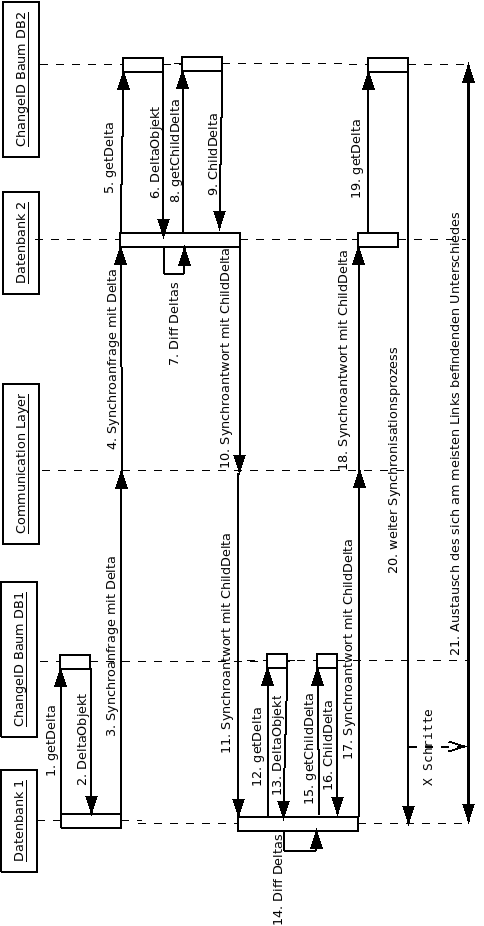
\includegraphics[width=1\textwidth]{bilder/SynchroProzess.png}
    \caption{UML Sequenzdiagramm des Synchronisationsprozesses}
\end{figure}
Durch ein Vergleichen der IDs und \enquote{Change IDs} in den sich synchronisierenden Datenbanken kann einfach festgestellt werden, welche Daten fehlen und, falls ein Datensatz vorhanden, auf welcher Seite dieser aktueller ist. Ein Vergleichen der gesamten Datenbanken, gerade wenn diese unter hoher Last stehen und sehr viele Datensätze verwalten, beansprucht jedoch viele Ressourcen. Ab einem gewissen Grad von Last durch Operationen und Masse an Daten ist dies nur noch schwer umsetzbar. Ein komplettes Abgleichen nimmt in diesem Fall so viel Zeit in Anspruch, dass durch neue Operationen wieder ein Ungleichgewicht zwischen den Datenbanken entstehen würde.\\\\
Daher gilt es, eine Synchronisationsmethodik zu finden, die sowohl in der Lage ist, schnell kleine Unterschiede auszugleichen, als auch Datenbanken, die sich auf völlig verschiedenen Ständen befinden, über eine längere Zeitspanne zu synchronisieren.
Die \enquote{Change IDs}, die zum Vergleich während der Synchronisation gepflegt werden, werden in jeder Datenbank in einem \enquote{EB-Baum} gehalten. Die Möglichkeit des Vergleichens von Zweigen unterhalb jedes Knotens ist daher von großem Vorteil. Um dies möglich zu machen, wird für jeden Knoten eine, den Zustand seiner beiden Kindobjekte repräsentierende Nummer, die \enquote{Knoten Change ID}, errechnet.
 Dazu werden die Nummern der Kindobjekte, \enquote{Change IDs} falls das Kind ein Blatt oder \enquote{Knoten Change ID} falls das Kind ein Knoten ist, durch eine \enquote{binäre XOR Operation} verbunden. Während des Synchronisationsprozesses senden sich beide Seiten sogenannte \enquote{Deltas} zu. %TODO inser Describtion
 Diese enthalten eine die Position des Deltaknoten beschreibende Ganzzahl, die Bitebene des  Deltaknoten, der Bitebene des sich über dem Deltaknoten befindenden Elternknoten, sowie die deren Zustand wiedergebenden Nummern seiner Kinder.
Die übertragenen Werte beschreiben das logisch zusammenhängende Dreieck aus Knoten und zwei Kindern. Daher wird dieses als \enquote{Delta} bezeichnet.\\\\
\begin{figure}[h!]
  \begin{center}
    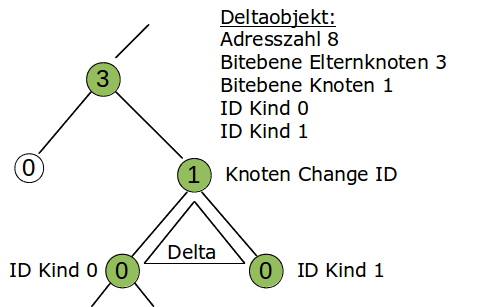
\includegraphics[width=.5\linewidth]{bilder/SynchroDelta.png}
  \end{center}
 \caption{Synchronisations Deltaobjekt}
\end{figure}
Durch die Ganzzahl, welche die Position des Deltas beschreibt, kann der Knoten, mit dem das Delta verglichen werden soll, in einer anderen Replikation gefunden werden. Bei der Lokalisierung des zu vergleichenden Knotens wird am obersten Knoten des Baumes begonnen und der Baum rekursiv durchlaufen. Je nachdem, ob 0 oder 1 in der binären Repräsentation der Adresszahl an Stelle des Ebenenbits des zu durchlaufenden Knoten gesetzt ist, wird das linke oder rechte Kindobjekt weiter behandelt. Dies wird solange wiederholt, bis die im Delta übergebene Bitebene des Deltaelternknoten unterschritten und der sich dort befindliche, zu vergleichende Knoten ermittelt ist.
Wird nach dem Vergleichen der Deltas festgestellt, dass die\enquote{Knoten Change IDs} der linken Knoten gleich und die der rechten Knoten ungleich sind, soll dieser Knoten ab jetzt nach rechts durchlaufen werden. Dazu wird in der binären Repräsentation des Adresswertes an der Bitstelle, die der Knoten darstellt, eine 1 gesetzt. Von nun an wird bei allen weiteren Durchläufen dieses Synchronisationsprozesses an diesem Knoten das rechte Kindobjekt behandelt.
Die Synchronisation kann von jeder Replikation angestoßen werden. Eine Möglichkeit, dies zu koordinieren, ist, dass jede Replikation zufällig in einem festgelegtem Zeitintervall zu synchronisieren beginnt. Es ist möglich, dass sich die Replikation während des Synchronisationsprozesses verändert. Die Synchronisation besteht aus zwei Phasen.  
\subsection{Synchronisation Phase 1} 
In der Ersten Phase gilt es, den Unterschied zu finden, der sich in beiden Bäumen am weitesten links befindet und somit den ältesten Unterschied zwischen den Replikationen darstellt. Da im laufenden Betrieb auf der rechten Seite des Baumes viel Veränderung stattfindet, soll immer der Unterschied, der davon am weitesten Entfernt liegt, zu erst ausgeglichen werden. Daten, die sich oft verändern, sind sehr weit rechts im Baum zu finden. Somit besteht die Chance, dass sich möglicherweise verlorene Veränderungen bei einer erneuten Veränderung selbst ausgleichen.
Die Datenbank, die mit der Synchronisation beginnt, sendet ein Delta des höchsten Knotens, gekapselt in einer Synchronisationsanfrage, an die andere Datenbank. Diese lokalisiert den Knoten mit dem das Delta abgeglichen werden soll und vergleicht die Nummer des linken Kindobjektes des erhaltenen Deltas mit dem linken Kindobjekt des eigenen Knotens. Sind diese gleich, werden die rechten Kindobjekte verglichen. Wird dabei kein Unterschied erkannt, sind die Datenbanken synchron und der Synchronisationsvorgang ist abgeschlossen. Falls aber ein Unterschied lokalisiert wurde, wird darauf mit einem Delta, bestehend aus dem sich unterscheidenden Kindobjekt, geantwortet. Die Datenbanken spielen im Synchronisationsprozess mit dem Senden der Deltas eine Art \enquote{Ping-Pong}, bis der am weitesten links liegende Unterschied gefunden wurde.\\\\
Beim Abgleichen der Deltas kommt es zu unterschiedlichen Vergleichsfällen, die vom Synchronisationsalgorithmus separat behandelt werden müssen.
\subsubsection{Unterschied Links/Rechts}
\label{sssec:SynchroDiffLeftOrRight}
Die Knotenstruktur in den \enquote{Change ID-Bäumen} beider Datenbanken ist bis zum ersten Unterschied identisch. Der Synchronisationsalgorithmus läuft Delta für Delta die Bäume entlang und navigiert dabei, nach links oder rechts abhängig davon an welcher Stelle sich \enquote{Knoten Change Ids} unterscheiden, bis ein Blatt gefunden wird. Es besteht aber nun die Möglichkeit, dass sich an der Stelle, an der das Blatt gefunden wurde, im anderen Baum ein Zweig befindet, in dem das Blatt bereits vorhanden ist, \autoref{fig:Case1TreeB,B*}. Beim Vergleichen der \enquote{Change IDs} wird in diesem Fall ein Unterschied festgestellt, doch befindet sich dieser im Unterzweig der anderen Datenbank. Bevor dieser aber lokalisiert werden kann, wird in der Datenbank ohne den Unterzweig bereits dass Blatt gefunden. Daher wird sobald ein Blatt gefunden wird, dessen ID der anderen Seite mitgeteilt und dort geprüft ob diese bereits vorhanden ist. Falls das Blatt noch nicht vorhanden ist, werden nun die kompletten Daten des Blattes angefordert und eingefügt.\begin{wrapfigure}{r}{0.5\textwidth}
  \begin{center}
    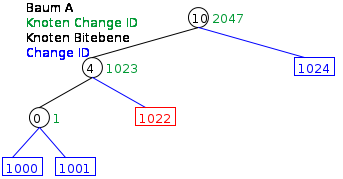
\includegraphics[width=0.9\linewidth]{bilder/Case1TreeA.png}
  \end{center}
 \caption{Baum A}
 \label{fig:Case1TreeA}
\end{wrapfigure} Ist das Blatt aber bereits im Baum, wird an die Position des Unterzweigs gelaufen und dort das Blatt betrachtet, welches sich am weitesten links befindet. Ist dieses nicht das gefundene Blatt, wurde der sich am weitesten links befindende Unterschied gefunden und der Datensatz zum Einfügen an die andere Datenbank gesandt. Ist das sich am weitesten links befindliche Blatt allerdings das Gefundene, ist der sich am weitesten links befindende Unterschied der nächste rechte Nachbar und kann ausgetauscht werden.
\begin{figure}[h!]
  \begin{center}
    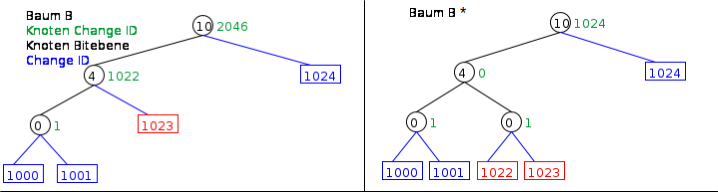
\includegraphics[width=0.9\linewidth]{bilder/Case B Baeume.png}
  \end{center}
 \caption{Baum B, B*}
  \label{fig:Case1TreeB,B*}
\end{figure}
\subsubsection{Behandeln von unterschiedlichen Baumtiefen} 
Abhängig davon, wie sehr sich die Bäume unterscheiden, so verschieden ist auch die Struktur an Knoten. Das führt zu folgender Problematik: Der älteste gesuchte Unterschied liegt links im Baum, doch fehlen ebenfalls andere, neuere Werte und somit auch die Knoten, die mit ihnen erzeugt werden. Ein einfaches \enquote{Delta Ping-Pong} Knoten für Knoten, und dabei Bitebene für Bitebene, ist daher nicht möglich. Auch ist von der Möglichkeit auszugehen, dass auf beiden Seiten Bitebenen fehlen. Dies führt zu einer Vielzahl an Möglichkeiten, in denen sich beiden Seiten unterscheiden können. Um die Lücken an Knoten zu erkennen und zu behandeln ist in den Deltaobjekten die Bitebene des Deltaknoten, sowie die Bitebene des oberhalb liegenden Elternknoten, enthalten.\\\\
Zu Beginn eines Synchronisationsschrittes wird im Baum der Knoten ermittelt, welcher sich unterhalb der Bitebene des Elternknotens des erhaltenen Deltas befindet. Dazu wird der Baum mit der Adresszahl solange durchlaufen, bis die Bitebene des betrachteten Knotens, die Bitebene des Elternknotens des erhaltenen Deltas unterschreitet. Nun wird geprüft, ob die Bitebene des gefundenen Knotens gleich der Bitebene des erhaltenen Deltaknotens ist. Ist dies der Fall, wird mit der im oberen \autoref{sssec:SynchroDiffLeftOrRight}, Unterschied Links/Rechts, beschriebenen Prozedur verfahren. Unterscheiden sich die Bitebenen, führt dies zu zwei Möglichkeiten 
\begin{figure}[h!]
  \begin{center}
    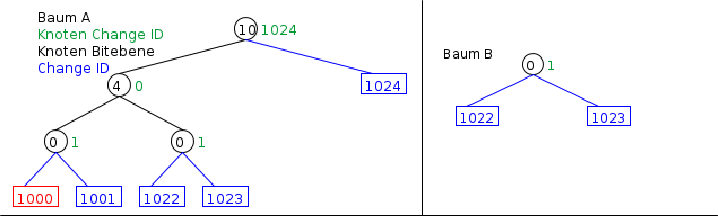
\includegraphics[width=0.9\linewidth]{bilder/case 2 a* B**.png}
  \end{center}
 \caption{Bäume mit verschieden vielen Bitebenen}
\end{figure}\\
\underline{{\bf Erste Möglichkeit:}} Die Bitebene des gefundenen Knotens ist kleiner als die des Deltaknotens. Zwischen den beiden Knoten befindet sich ein Loch, in dem sich noch nicht synchronisierte Blätter, sowie dazugehörige Knoten befinden. Diese sollen jedoch erst später vom Algorithmus repariert werden, da diese neuer sind und zuerst der älteste Unterschied behoben werden soll. Daher gilt es, das Loch zu überspringen. Dazu sendet die Seite mit dem tieferen Knoten ein spezielles Delta zurück, welches das nächst linke Delta unterhalb des erhaltenen Deltas anfordert. Dies wird solange wiederholt, bis auf beiden Seiten die selbe Bitebene erreicht ist, bzw. falls die kleine Bitebene im anderen Baum nicht vorhanden ist, ein Blatt gefunden wird. Ist auf beiden Seiten die gleiche Bitebene erreicht, können die Kinderobjekte, wie im obigen \autoref{sssec:SynchroDiffLeftOrRight} beschrieben, verglichen werden.\\\\
\underline{{\bf Zweite Möglichkeit:}} Falls aber die Bitebene des gefundenen Knotens größer ist, als die des Deltaknotens, wird ein Delta aus dem gefundenen Knoten gebildet und zurück gesandt. Damit werden einfach die Seiten getauscht und der gerade beschriebene Fall tritt ein. Diese Methodik wird ebenfalls genutzt, um mit Synchronisation zu beginnen. Einer der Datenbanken wird ein manipuliertes Deltaobjekt gesandt. Dieses trägt als Absender die andere Datenbank. Die Werte der Bitebenen von Deltaknoten und Elternknoten sind negativ. Somit wird zuerst der oberste Knoten lokalisiert. Da dessen Ebenenbit positiv und somit größer ist, als der erhaltene negative Deltawert, wird der oberste Knoten als Delta an die andere Datenbank gesandt und ein Synchronisationsschritt beginnt. \\\\
\begin{figure}[h!]
  \begin{center}
    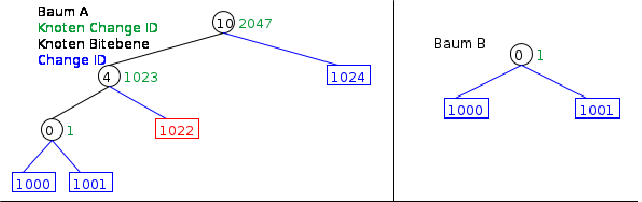
\includegraphics[width=0.9\linewidth]{bilder/case 2 A B1.png}
  \end{center}
 \caption{Bäume mit verschieden vielen Bitebenen}
\end{figure}
Ein weiterer Sonderfall tritt ein, wenn der Knoten und seine unter ihm liegenden Kinder des Baumes mit fehlenden Knoten im anderen Baum bereits vollständig enthalten ist und sich der gesuchte Unterschied oberhalb davon befindet. Während des Angleichens der Bitebenen werden keine \enquote{Change IDs} verglichen. Erst wenn auf beiden Seiten die selbe Bitebene erreicht ist, wird wieder nach Unterschieden geprüft. Wenn in diesem Fall links und rechts keine Unterschiede gefunden werden, erscheinen die Bäume synchron. Daher muss beim Überspringen des Bitebenenlochs überprüft werden, ob dieses bereits die selbe \enquote{Change ID}  hat wie der Knoten, bevor das nächst tiefere Delta angefordert wird. Ist dies der Fall, liegt der gesuchte Unterschied ganz links im rechten Kindobjektzweig, oder ist das Kindobjekt selbst.

\subsection{Synchronisation Phase 2}
Nach Ablauf der ersten Synchronisationsphase ist die sich, in den \enquote{Change-ID Bäumen}, am weitesten Links befindende, unterscheidende \enquote{Change-ID} gefunden. Nun sendet die Datenbank in der sich diese befindet das gesamte \enquote{EbTreeDataObjekt} auf welches die \enquote{Change-ID} referenziert an die andere Datenbank in der diese \enquote{Change-ID} nicht vorhanden ist. Durch die im \enquote{EbTreeDataObjekt} enthaltene ID kann nun im  \enquote{ID-Baum} geprüft werden ob diese enthalten ist. Falls dies nicht der Fall ist, ist die komplette Einfügeoperation des Datensatzes verloren gegangen und dieser muss nun nachträglich in beide Bäume eingefügt werden. Ist es Möglich die ID zu lokalisieren ist dass \enquote{EbTreeDataObjekt} bereits in beiden Datenbanken vorhanden aber auf einem unterschiedlichem Stand. Nun gilt es durch einen Vergleich der beiden \enquote{Change-IDs} heraus zu finden auf welcher Seite der Datensatz aktueller ist und dies auszugleichen. Ist die erhaltene \enquote{Change-ID} größer als die Eigene wird der eigene Datensatz aktualisiert. Ist aber die erhaltene \enquote{Change-ID} kleiner kann der eigene Datensatz als Update an die andere Datenbank gesandt werden. Der Synchronisationsschritt ist abgeschlossen. Egal ob eine veraltete oder aktuelle  \enquote{Change-ID} gefunden wird, jeder Synchronisationsschritt führt zum Ausgleich eines Unterschiedes.

\subsection{Aufwand der Synchronisation}
Alternativ zu der im vorherigen Absatz beschriebenen Synchronisationsmethodik kann eine Synchronisation durch das Vergleichen aller Datensätze die in den beteiligten Knoten abgelegt sind erfolgen. Durch das Senden und Vergleichen von Inhalthashes ist es Möglich die gesuchten Inkonsistenzen zu lokalisieren und Auszugleichen. Jedoch müssen dabei alle Elemente der an der Synchronisation beteiligten Knoten verglichen werden, was eine Komplexität von 2 * Anzahl aller Elemente zur Folge hat. Der im vorherigen Absatz beschriebene Synchronisationsalgorithmus verfolgt einen differenzierteren Ansatz und muss nicht alle Elemente vergleichen sondern ist in der Lage Inkonsistenzen direkt aufzuspüren. Daher ist seine Komplexität log(n) *  Anzahl der Inkostitenzen. In diesem Absatz soll daher die Komplexität beider Ansätze verglichen und bewertet werden \footnote{In Kooperation mit der SpinningWheel GmbH erstellte Komplexitätsskizze}.
\begin{description}
   \item[n ] Anzahl aller sich im System befindlichen einzigartigen Elemente
   \item[p] Grad an Unterschied 
\end{description}

Um beide Ansätze zu Vergleichen wird die Anzahl an Vergleichsoperationen bei verschiedenen Graden an Unterschied berechnet. In diesem Beispiel befinden sich 10.000 einzigartige Datensätze, Variable n, im verteilten Datenbanksystem.

\begin{table}[h!]
\centering
    \begin{tabular}{| l | l | l | l | l |}
    \hline
    Komplexität & 1\% Unterschied p & 10\% Unterschied p & 20\% Unterschied p & 100\% Unterschied p\\ \hline
    log(n) * p * n & 1329 & 13288 & 26575 & 132877 \\ \hline
    2 * n & 20.000 & 20.000 & 20.000 & 20.000\\ \hline
    \end{tabular}
\caption{Anzahl benötigter Vergleichsoperationen zweier Synchronisationsansätze bei 10.000 Datensätzen}
\label{table:1}
\end{table}

Aus dem Beispiel wird schnell ersichtlich das die Leistung der in dieser Arbeit entwickelten Synchronisationsmethodik am besten ist, je geringer der Unterschied zwischen den sich unterscheidenden Knoten ist. Ab einem Grad von 20\% Unterschied ist sie sogar schlechter als ein komplettes Abgleichen beider Knoten.
	
\section{Architektur des Prototypen}
\begin{figure}[h!]
  \begin{center}
    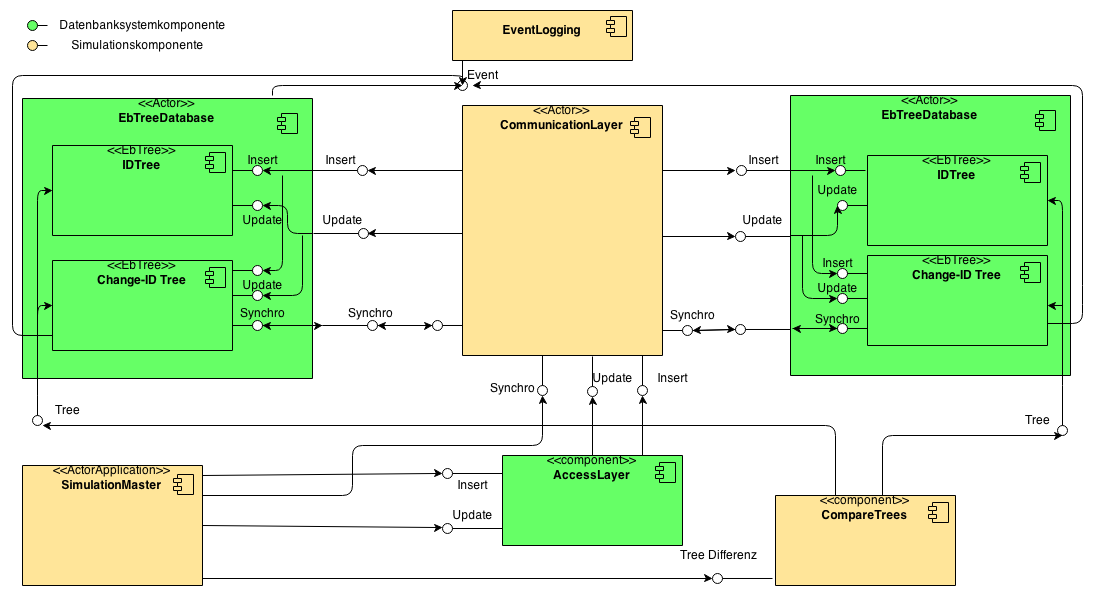
\includegraphics[width=1.0\linewidth]{bilder/prototyp_component_diagram.png}
  \end{center}
 \caption{UML Komponentendiagramm des Prototypen}
\end{figure}
\todo[inline]{ turn picture}
Der in dieser Arbeit erstellte Prototyp besteht grundlegend aus zwei Teilen. Zum einen besteht er aus den Komponenten des in \autoref{sec:DBConcept} beschriebenen Datenbankkonzeptes und der in \autoref{sec:eBTreeSynchronisation} erklärten Synchronisation zwischen zwei Instanzen der Datenbank. Zum anderen besteht er aus einer Simulationsumgebung, mit welcher die Funktionalität des Datenbanksystems getestet werden kann. Die Synchronisation zwischen den einzelnen Datenbankinstanzen kann hier ebenfalls getestet und analysiert werden. Durch verschiedene Initialisierungen des Datenbanksystems, sowie dem Erzeugen von Last, können verschiedene Szenarien erzeugt, und die Leistung des Systems bewertet werden. \\
Die Applikation ist zum Teil als Actorsystem umgesetzt. So wird jede Datenbank, sowie auch der \enquote{CommunicationLayer}, welcher als Bindeglied zwischen den Komponenten fungiert, durch einen Aktor repräsentiert.
Das Senden von Actornachrichten ähnelt dem Senden von IP-Paketen zwischen zwei Datenbanken an verschiedenen Standorten. Wann welche Nachricht in welcher Reihenfolge bei welcher Datenbank ankommt ist nicht vorhersehbar. Verlust, sowie Verspätung von Paketen und die daraus resultierende Asynchronität der Datenbanken, lassen sich so gut simulieren.
Zwischen den Datenbankaktoren befindet sich, als Teil der Simulationsumgebung, eine Kommunikationsebene. In dieser können Verlust und Verspätung von Paketen gesteuert werden.


\subsection{Datenbankkomponenten}
Der Prototyp setzt einen Teil der, in \autoref{sec:DBSystemConcept} beschriebenen, Komponenten um. Die Generierung von IDs, welche neue Daten adressieren und den Stand von Aktualisierungen abbilden, werden in einer Basisimplementierung des \enquote{Accesslayer} generiert. Diese werden mit den Daten in einem \enquote{EbTreeDataObjekt} gekapselt und an alle Datenbankzellen gesandt. Jede Datenbankzelle wird durch einen Actor repräsentiert und kann Nachrichten mit neuen Daten, Änderungen oder Synchronisationsanfragen erhalten und senden. Im Rahmen dieser Arbeit werden zwei Datenbankzellen verwendet und die Operationen Einfügen und Aktualisieren, sowie die Synchronisation zwischen beiden, getestet. Die Datensätze werden in einer Erweiterung des klassischen \enquote{EB-Baum} gehalten.

\subsection{Simulationskomponenten}     
Die Komponenten der Simulationsumgebung setzen auf den Datenbankkomponenten auf. Zwischen den zwei Datenbankknoten und dem \enquote{Accesslayer} wird der \enquote{CommunicationLayer} geschoben. Der \enquote{CommunicationLayer} ist, wie die zwei Datenbankknoten, ein Actor. Werden neue Daten eingefügt oder aktualisiert, werden diese vom \enquote{Accesslayer} an den \enquote{CommunicationLayer} übergeben und an die zwei Datenbanken weiter verteilt. Auch die Synchronisation zwischen den beiden Knoten läuft durch den \enquote{CommunicationLayer}. Die Daten, die im Datenbankystem gekapselt in \enquote{EbTreeDataObjekten} oder \enquote{Deltaobjekten} versandt werden, werden als Nachrichten zwischen den Actoren versandt. Jede Nachricht passiert den \enquote{CommunicationLayer} und kann somit in diesem beeinflusst werden. So kann ein Prozentwert eingestellt werden, mit dem Pakete verloren gehen, um das Senden von UDP-Paketen zu simulieren. Auch die Verzögerung von Paketen kann hier simuliert werden. Neue Datensätze oder Aktualisierungen alter Daten werden in einer \enquote{Queue} abgelegt. Soll ein Paket verzögert werden, wird es lediglich, abhängig davon, wie stark die Verzögerung sein soll, weiter hinten eingereiht und somit später versandt. Durch Verlust und Verzögerung werden die Datenbestände in beiden Replikationen verschieden. Je nachdem, wie hoch Verzögerung und Verlust im \enquote{CommunicationLayer} eingestellt sind, können in anderen Teilen der Simulationsumgebung die Auswirkungen auf das gesamte System und die Synchronisation ermittelt werden.\\\\
Startpunkt der Simulationsumgebung, als auch des gesamten Prototypen, ist der \enquote{SimulationMaster}. In dieser Komponente wird beim Start des Prototypen das Actorsystem initialisiert. Die beiden Datenbankzellen, \enquote{Accesslayer} und \enquote{CommunicationLayer}, werden instanziiert, deren Referenzen unter den Komponenten ausgetauscht und das gesamte Datenbanksystem, sowie die Simulationsumgebung selbst, initialisiert. Aufgabe des \enquote{SimulationMaster} ist es, zum einen das System zu initialisieren und zu starten, zum anderen darauffolgend eine Reihe verschiedener Simulationen zu ermöglichen. Während der Simulation werden Daten ausgewertet und diese in einer CSV-Datei gespeichert. Welche Simulation ausgeführt werden soll, kann von dem\_r Nutzer\_in  in einem einfachen \enquote{Kommandozeileninterface} ausgewählt werden. Je nach Simulation wird nun das Datenbanksystem mit Daten initialisiert und mit der Simulation begonnen. Während der Simulation kann der Inhalt der einzelnen Zellen verändert werden, um Last auf das Datenbanksystem zu simulieren. Der \enquote{SimulationMaster} generiert dazu Änderungen und sendet diese, via des \enquote{AccessLayers}, an den \enquote{CommunicationLayer}. Dort wird nun entschieden, ob das Paket verloren geht oder verspätet wird. Anschließend wird dieses in der \enquote{Queue} abgelegt. Der \enquote{SimulationMaster} sendet in gewissen festgelegten Intervallen ein \enquote{Clocksignal}, welches dafür sorgt, dass die Pakete im ersten Feld der \enquote{Queue} versandt werden. Davon abhängig, wie hoch der Verlust oder die Verspätung von Paketen eingestellt ist, ergibt sich ein Unterschied zwischen den Knoten, der mit der Synchronisation ausgeglichen werden soll. Die Synchronisation der Datenbankknoten wird ebenfalls im \enquote{SimulationMaster} gestartet. Dazu wird an den \enquote{CommunicationLayer} die Nachricht gesandt, dass mit der Synchronisation eines Unterschiedes begonnen werden soll. In der Nachricht ist enthalten, welche Datenbank mit der Synchronisation beginnt. Der \enquote{SimulationMaster} wartet nun bis die Synchronisation eines Unterschiedes abgeschlossen ist und fährt dann mit der Simulation fort.\\\\

Um den Erfolg der Synchronisation und das Entstehen von Unterschieden bestimmen zu können, existiert die Komponente \enquote{TreeCompare}, mit welcher der Unterschied beider Replikationen bestimmt werden kann. Um den Unterschied zu bestimmen, werden die \enquote{ID-Bäume} und \enquote{Change ID-Bäume} beider Datenbankreplikationen Blatt für Blatt verglichen und es wird gezählt, um wie viele Elemente sich diese unterscheiden. Beim Vergleichen der \enquote{ID-Bäume} kann festgestellt werden, um wie viele Einfügeoperationen und beim Vergleichen der \enquote{Change ID-Bäume} , um wie viele Aktualisiersoperationen sich beide Datenbanken unterscheiden.

%TODO eventlogging
%---------------------------------------------------------------------------------------------------------------------------------------------------
\chapter{Implementierung}

\section{EBTree} % teil gurndlage teil implementation
\label{sec:EbTreeImpl}
Die im Rahmen dieser Arbeit erstellte Scalaimplementierung des \enquote{Elastischen Binärbaums} orientiert sich sowohl an dem, in Grundlagen~\ref{sec:ebTreeGrundlagen} beschriebenen, Entwurf von Willy Tarreau\autocite{Tarreau}, als auch auf einer mehr spezifischen Basisumsetzung der \enquote{SpinningWheel GmbH}.\\
In der nachfolgend beschriebenen Implementierung  wird bereits die enge Koppelung von Knoten und Blättern der ursprünglichen C Implementation aufgebrochen. Die von Tarreau in \enquote{C structs} aufgebauten Knoten und Blätter wurden von \enquote{SpinningWheel GmbH} durch Java Klassen ersetzt und ihre gemeinsamen Eigenschaften in einem Interface definiert. Basisfunktionen des Baumes,wie das Einfügen, Löschen und Durchlaufen des Baumes, waren hier ebenfalls vorhanden und wurden als Teil der Arbeit in Scala neu umgesetzt.\\\\
Eine besondere Anforderung an den Baum ist, dass die sortierten und verwalteten Schlüssel einzigartig sind und ein Einfügen von Duplikaten verhindert wird. Da das Verwalten von Duplikaten an sich möglich, aber für das Funktionieren des Baumes nicht zwingend notwendig ist, wird ein Einfügen von Duplikaten in der anschießend beschrieben Umsetzung vermieden. \\
\subsection{Grundlegender Aufbau}
Der Baum selbst wird durch eine generischen Klasse gekapselt. Diese besteht aus den Funktionalitäten des Baumes, zwei \enquote{Case-Klassen}, die Knoten und Blätter repräsentieren, sowie einem \enquote{Trait}, der die gemeinsame Eigenschaften von Knoten und Blatt beschreibt. Der generische Typ der Klasse wird bei der Instanziierung von Knoten oder Blatt übergeben und legt den Datentyp der in den Blättern gespeicherten Daten fest. Somit kann der Baum jede Art von Daten halten, ohne verändert werden zu müssen.\\

Der \enquote{Trait} Child beschreibt, was das \enquote{Kind} eines Knotens können muss. Ganz gleich, ob es sich hier um ein Blatt oder einen weiteren, einen neuen Zweig öffnenden, Knoten handelt. Festgelegt ist, dass ein jedes \enquote{Kindobjekt} eine Referenz auf ein \enquote{Elternobekt} haben muss und eine Methode, die eine eindeutig identifizierbare ID des Objektes zurück gibt. Bei Blättern ist die ID der Schlüssel, mit dem das Blatt eingefügt wird und bei Knoten ist es die \enquote{Node Change ID}, welche zum Vergleichen von Baumzweigen anderer Datenbanken bei der Synchronisation verwendet wird.Durch den Einsatz von \enquote{Case-Klassen} und \enquote{Pattern Matching} beim Durchlaufen des Baumes kann sehr einfach geprüft werden, welcher Klasse Kindelemente angehören. \\

Die Aufgabe des Blattes \enquote{Case Klasse} ist sehr einfach: Sie hält die Referenz auf einen übergeben Datensatz und ist durch einen eindeutigen Schlüssel identifizierbar. Knoten hingegen beinhalten mehr Logik.  So kann ein Knoten die in seiner Wurzel gespeicherten Kindobjekte, Zweige oder Blätter, zurück geben oder neue anfügen. Durch sein Ebenenbit weiß ein Knoten auf welcher binären Ebene des Baumes er sich befindet und kann in dem Schlüssel, der bei einer Abfrage- oder Einfügeoperation übergeben wird, an der entsprechenden Stelle nachschauen und seinen linkes oder rechtes Kindobjekt verarbeiten.

\begin{listing}[H]
	\begin{minted}[mathescape,
	               numbersep=5pt,
	               frame=lines,
	               framesep=1mm]{scala}
case class Node[T](myBit: Int) extends Child[T] {
    var myZero:				Child[T]  = _
    var myOne:				Child[T]  = _
    var nodeChangeID:	Long    	= _

    def bitOne(uid: Long): Boolean = ((uid & (1L << myBit)) != 0) && (myBit < 64)

    def getChild(uid: Long): Child[T] = bitOne(uid) match {
      case true => myOne;
      case false => myZero
    }
    def setChild(uid: Long, child: Child[T]) = {
      bitOne(uid) match {
        case true => myOne = child
        case false => myZero = child
      }
      child.myParent = this
    }
    override def getID(): Long = nodeStateID
  }	
	\end{minted}
	\caption{Umsetzung eines Knoten des \enquote{EB-Baum}}
	\label{lst:Knoten EB-Baum}
\end{listing}

\subsection{Funktionalität des Baumes}
\subsubsection{Finden von Schlüsseln}
\label{sssec:FindKey}
Die Suche eines Schlüssels ist durch schlanke rekursive Funktion gelöst. Der zu suchende Schlüssel gibt eine Art binären Weg vor. So beginnt die Funktion am ersten Knoten des Baumes. Diesem wird der zu suchende Schlüssel übergeben. Der Knoten weiß durch sein Ebenenbit, welche Stelle er in binären Repräsentation des Schlüssels einnimmt. Je nachdem, ob das Bit an dieser Stelle 0 oder 1 ist, gibt er sein linkes oder rechtes Kindobjekt zurück. Nun kann via \enquote{Pattern Matching} unterschieden werden, ob es sich bei diesem um einen weiteren Knoten, oder ein Blatt handelt. Ist das gefundene Objekt ein Blatt, wird die Rekursion abgebrochen und das Blatt zurück gegeben. Falls ein Blatt mit dem gesuchten Schlüssel im Baum vorhanden ist, wird dieses, falls nicht, das Blatt mit am dem nächst kleinerem Schlüssel, beim durch laufen des Rekursion gefunden. Falls das gefundene Objekt aber ein Knoten ist, der einen neuen Zweig öffnet, wird mit diesem die rekursive Funktion erneut aufgerufen, bis ein Blatt gefunden wird.
\subsubsection{Einfügen eines neuen Blattes}
Beim Einfügen eines neuen Blattes wird der Baum zunächst nach dem Schlüssel des neuen Blattes durchsucht. Falls der Schlüssel bereits vorhanden ist, wird der neuen Datensatz im gefundenen Blatt eingefügt und der alte Datensatz zurückgegeben. So wird verhindert, dass Duplikate eingefügt werden können. Falls der Schlüssel nicht vorhanden ist und sich bereits Blätter im Baum befinden, liefert die Methode, die für das Suchen von Blättern zuständig ist, das Blatt, dessen Schlüssel die dem gesuchten Schlüssel ähnlichste binäre Repräsentation besitzt. Nun werden die Schlüssel des neuen und des gefundenen Blattes durch eine binäre Oder-Operation verknüpft und die Bitstelle des höchsten Bitunterschiedes ermittelt. Diese wird das neue Ebenenbit des Knotens, der mit dem Blatt eingefügt wird. Nun muss die passende Ebene im durch die Suche ermittelten Zweig gefunden werden. Dazu wird das Ebenenbit des Elternknoten des gefundenen Blattes mit dem neu bestimmten Ebenenbit verglichen. Ist das neue Ebenenbit kleiner als Ebenenbit des Elternknoten, wurde die richtige Ebene gefunden. Andernfalls wird der Zweig Knoten für Knoten von unten nach oben durchlaufen, bis die passende Stelle gefunden ist. An dieser kann dann der neue Knoten samt Blatt eingehängt werden. Das Durchlaufen dieses Algorithmus stellt sicher, dass ein neuer Schlüssel stets an der richtigen Stelle eingefügt wird und der Baum aufsteigend von links nach rechts sortiert ist.
\subsubsection{Entfernen eines Blattes}
Soll ein Blatt aus dem Baum entfernt werden, wird es zunächst lokalisiert. Dazu wird der Baum nach dem Schlüssel des zu löschenden Blattes durchsucht. Nachdem die Referenz des Blattes gefunden wurde, gilt es nun, sowohl das Blatt, als auch den sich darüber befindenden Elternknoten, zu entfernen. Dazu wird das andere Kindobjekt, welches neben dem zu löschendem Blatt existiert, im Elternknoten des  zu löschendem Knoten an dessen Position gehängt. Da nun kein Objekt mehr auf den Elternknoten referenziert, werden dieser und das zu löschende Blatt beim nächsten Durchlauf der \enquote{Garbage collection} gelöscht. Anschließend wird der Zähler, der die Anzahl der Blätter im Baum hält, dekrementiert und der Inhalt des gelöschten Blattes zurück gegeben.
\subsubsection{Erzeugen von Knoten Status IDs}
Das Vergleichen von Blättern ist durch deren einzigartigen, aufsteigenden Schlüssel einfach umzusetzen. Bei dem in dieser Arbeit umgesetzten Synchronisationansatz, siehe \autoref{sec:eBTreeSynchronisation}, muss es aber möglich sein, ganze Zweige unterhalb eines Knotens zu vergleichen. Daher besitzt der Baum eine Funktion, die es ermöglicht für jeden Knoten eine Nummer, die \enquote{Knoten Status ID}, zu erzeugen. Diese repräsentiert den Zustand seiner beiden Kinder.\\ Wird ein Blatt angefügt oder gelöscht, werden die \enquote{Knoten Change ID} rekursiv nach oben bis zur Wurzel generiert. Für den Fall, dass das Blatt neu eingefügt wurde, beginnt die Rekursion am neu eingefügtem Knoten. Wird aber ein Blatt gelöscht, beginnt die Rekursion am Knoten oberhalb mit dem Blatt gelöschtem Knoten. Nun wandert die Rekursion Elternknoten für Elternknoten bis zur Wurzel des Baumes. Auf dem Weg wird für jeden Knoten eine neue \enquote{Knoten Change ID} generiert. Dabei werden die IDs der Kindobjekte des zu dem Zeitpunkt behandelten Knotens durch eine binäre XOR-Operation verknüpft und der Wert im Knoten gespeichert. Ist das Kindobjekt ein Blatt, wird als ID der Schlüssel verwendet. Ist das Objekt ein Knoten, wird seine bereits berechnete \enquote{Knoten Status ID} verwendet.
\subsubsection{Methoden zur Synchronisation und das Deltaobjekt}
Um die, in \autoref{sec:eBTreeSynchronisation}, beschriebene Synchronisation zu realisieren, wird die nach Scala portierte Version des \enquote{EB-Baum} um zwei Methoden erweitert. Um den \enquote{Ping-Pong-artigen} Austausch von Deltaobjekten zwischen den Datenbanken zu ermöglichen, muss der Baum eine Methode besitzen, die zu einem gegeben Deltaobjekt das nächst passende Objekt ermittelt. Zu Beginn wird in der Methode \enquote{nextDelta} der Knoten gesucht, mit dem das erhaltene Delta verglichen werden soll. Dazu wird der Baum mit einer Rekursion von oben beginnend Knoten für Knoten durchlaufen. Dies erfolgt bis entweder ein Blatt gefunden, oder der Knoten ermittelt wurde, dessen Bitebene unterhalb derer des erhaltenen Deltaelternknotens liegt. Die Navigation, die festlegt, ob nach links oder rechts am Knoten abgebogen werden soll, funktioniert genau wie beim Suchen eines Blattes. Der Knoten hält dafür eine Methode bereit, die zu einem gegebenen Schlüssel, hier die Adresszahl des erhaltenen Deltas, das entsprechende Kind zurück gibt. Dazu betrachtet der Knoten das Bit an der Stelle seines Ebenenbits in der binären Repräsentation des Schlüssels und entscheidet welches Kindobjekt zurück gegeben wird. Es wird solange ein nächstes Delta angefordert, bis eine Seite ein Blatt entdeckt. Die nachfolgend beschriebene Vergleichslogik der Knoten entscheidet nur, wie im Baum navigiert wird, um am Ende ein Blatt zu lokalisieren.\\

Wird nun ein Blatt gefunden, wird dies der anderen Seite mitgeteilt. Dazu wird ein anderes, speziell initialisiertes, Deltaobjekt übertragen, welches dieses als Blatt identifizierbar macht. Um die verschiedenen Zustände der Klasse Delta erstellen zu können, besitzt diese ein \enquote{Companien Object}, welches als \enquote{Factory} fungiert und, je nach dem ob ein Blatt oder Knoten übergeben wird, ein verschieden initialisiertes Delta zurück gibt. Bildet ein Delta ein Blatt ab, sind die Werte für das rechte und linke Kindobjekt die ID des Blattes, sowie die Knoten Bitebene -1. Die Adresszahl und die Bitebene des Elternknotens bleiben erhalten und ermöglichen es immer noch die Position des Blattes nachzuvollziehen. Die Klasse Delta besitzt eine Methode mit der abgefragt werden kann, ob das Delta ein Blatt abbildet oder nicht.\\\\
\begin{listing}[H]
	\begin{minted}[mathescape,
	               numbersep=5pt,
	               frame=lines,
	               framesep=1mm]{scala}
def nextDelta(t:Delta):Delta = {
var node:Node[T] = rekFuncFindNode(myRoot.get.myZero) // Rekursion finden des Knotens
  if (node.myBit == t.to) { // Bitebene identisch vergleiche Kindobjekte
      if (node.myZero.getID() != t.l) {
        return Delta(t.id, t.to, node.myZero)
      }else if(node.myOne.getID() != t.r) {
        return Delta(t.id+(1L<<node.myBit), t.to, node.myOne); /
      }else{ return null } // trees synchronized
  }else if (node.myBit > t.to) {        // flip sides
      return  Delta(t.id, t.from, node); 
  }else { // node.myBit < t.to
      if (t.l == node.getID()) return new Delta(t.id+(1L<<t.to), 0 , 0, -1, -1)
      return  Delta(t.id, t.from, node.myBit, -1, -1) // request next left Delta
  }
}
	\end{minted}
	\caption{Vergleichslogik von erhaltenen Delta mit entsprechenden Knoten}
	\label{lst:DeltaComp}
\end{listing}
Wird aber in der beschriebenen Rekursion statt einem Blatt, der erste Knoten unterhalb der Bitebene des Elternknotens des Deltas gefunden, kann dieser mit dem erhaltenem Deltaknoten verglichen werden. Falls die Bitbene des Deltas und des Knoten identisch ist, können die IDs der Kindobjekte verglichen werden. Unterscheiden sich die linken IDs, wird aus dem linken Kindobjekt des Knotens ein Delta gebildet. Sind diese gleich, werden die IDs des rechten Kindobjekte verglichen. Sind auch diese gleich, ist der Baum synchron. Die Methodik des Synchronisationsalgorithmus stellt hierbei fest, falls dieser Fall nicht im obersten Knoten eingetreten ist. Sind die rechten Kindobjekte unterschiedlich, wird an der Position der Bitebene des Knotens das entsprechende Bit in der binären Repräsentation der Adresszahl gesetzt. Dazu wird zur Adresszahl der Wert addiert, der das entsprechende Bit setzt.\\

 Wurde links oder rechts eine Differenz erkannt, wird aus dem entsprechendem Kindobjekt ein Delta erstellt und zurück gegeben. Das Kindobjekt wird durch das Interface Child abgebildet und kann Knoten oder Blatt sein. Die \enquote{Factory Methodik} der Deltaklasse bildet daher automatisch das passende Delta, egal ob das Kindobjekt ein Blatt oder Knoten ist und liefert dieses zurück.\\\\
Das in \autoref{sec:eBTreeSynchronisation} \enquote{Behandeln von verschieden vielen Bitebenen} beschrieben Problem (die Bitebene des Deltaknoten und gefundene Knoten unterscheiden sich) wird in der Implementation wie folgt umgesetzt: Ist die Bitebene des gefunden Knotens größer, wird aus diesem ein Delta gebildet und zurück gegeben. Dieses Delta wird dann im anderen Baum verarbeitet. Falls die Bitebene des zu vergleichenden Knotens kleiner ist als die des Deltas, wird vom anderen Baum das nächste vom erhaltenen Delta gesehene tiefere linke Delta angefordert. Dazu werden die Felder für die IDs der Kinder auf minus Eins gesetzt. Die Adresszahl und die Ebene des Deltaelternknoten bleiben gleich. Somit wird beim Rekursiven Suchen des Knotens im anderen Baum dort wieder der Deltaausgangsknoten gefunden. Durch eine Abfrage vor dem Vergleich der Bitbenen wird erkannt, dass die Felder der Kinder mit minus Eins belegt sind und somit dass das nächste linke Delta unterhalb des Knotens angefordert wurde. Dies wird wiederholt bis die Bitebenen identisch sind und ein Vergleich der Kinder möglich ist.\\\\
Am Ende der in \autoref{sec:eBTreeSynchronisation} beschriebenen Logik wird entweder ein Blatt gefunden, welches nicht in beiden Bäumen vorhanden ist, oder die Synchronisation beendet, da die Bäume gleich sind. Wird ein sich unterscheidendes Blatt gefunden und an die andere Datenbank gesendet, muss geprüft werden, ob dieses nicht bereits vorhanden ist. Dies ist, auf Grund des in \autoref{sec:eBTreeSynchronisation} \enquote{Unterschied Links/Rechts} bereits beschriebenen Sonderfalls, notwendig (siehe \autoref{fig:Case1TreeB,B*}). Bei diesem Sonderfall befindet sich das vermeintlich unterscheidende Blatt im anderen Baum, allerdings nur in einem tiefer liegendem Zweig. Daher wird eine weitere Methode, \enquote{checkIfLostLeafIsFound}, bereitgestellt, die prüfen kann, ob das Blatt im Baum vorhanden ist oder nicht. Wenn dies der Fall ist, kann die Methode das Blatt, das sich am weitesten links im Zweig befindet, lokalisieren. Dies ist mit Sicherheit nur auf einer Seite vorhanden, da auf der anderen an der Stelle des Zweiges nur ein Blatt ist und somit alle Blätter außer diesem fehlen. Die Methode bedient sich zu Beginn der in \autoref{sssec:FindKey} \enquote{Finden von Schlüsseln} beschrieben Logik. Kann zu dem gegebenen Schlüssel kein Blatt gefunden werden, ist dieser der Gesuchte sich am weitesten Links befindende Unterschied. Der erhaltene Schlüssel wird zurück gegeben. Ist der Schlüssel aber im Baum enthalten, wird zuerst der Knoten gesucht, der sich im Baum an der Stelle des Blattes befindet. Da im erhaltenen Deltaobjekt noch die Adresszahl und die Bitebene des Elternknoten des erhaltenen Blattes enthalten ist, kann der Baum wieder rekursiv von oben durchlaufen werden, bis der Zweig lokalisiert ist. Der Zweig wird nun bis zu dem Blatt durchlaufen, das sich am weitesten links befindet. Nun muss nur noch geprüft werden, ob dieses Blatt das bereits als Deltaobjekt erhaltene Blatt ist. Ist dies der Fall, wird das nächste rechte Blatt zurück gegeben. Falls nicht wird das gefundene sich ganz links im Zweig befindliche Blatt zurück gegeben. 

\section{EbTreeDatabase}
\subsection{Grundlegender Aufbau}
Die Klasse \enquote{EbTreeDatabase} implementiert den, in \autoref{sec:DBConcept} beschriebenen, Aufbau einer Datenbankzelle. Sie erweitert die Klasse Actor des \enquote{Akka Actor toolkit} \autocite{akka}. Kommunikation mit der Datenbankzelle erfolgt somit ausschließlich durch das Senden von Nachrichten. Die Klasse verfügt über keine öffentlich erreichbaren Methoden. Die Datenbank besitzt eine \enquote{Mailbox}, in der erhaltene Nachrichten abgelegt werden. In der zu überschreibenden Methode \enquote{receive} werden die Nachrichten definiert, die von der Datenbank verarbeitet werden sollen. Dies ist durch Scala Logik des \enquote{Pattern Matching} realisiert. Erhaltene Daten werden in diesem Datenbankprototyp in zwei Indexen abgelegt. Dazu werden die Daten in der Klasse \enquote{EbTreeDataObject} gehalten. Diese verfügt über ein Feld für die ID, ein Feld für die \enquote{Change-ID}, sowie eine Referenz auf die eigentlichen Daten. Der Datenbankklasse wird bei ihrer Instanziierung ein Datentyp übergeben, welcher den Typ der eigentlichen, im  \enquote{EbTreeDataObject} gekapselten, Daten festlegt. Durch diese Logik eines generischen Types kann jede Art von Daten in der Datenbank abgelegt werden. Die beiden Indexe in dieser Basisumsetzung der Datenbank werden durch den, in \autoref{sec:EbTreeImpl} beschriebenen \enquote{EB-Baum} realisiert. Die Datenbank hält zudem Referenzen zu den anderen im System existierenden Datenbankknoten, welche in einer Liste aus Actorreferenzen gehalten werden, sowie einer Referenz auf den für die Simulation im Prototypen essentiellen \enquote{CommunicationLayer}.\\
\subsection{Verarbeitung von Nachrichten}
Bei den in der Datenbank verarbeiteten Nachrichten handelt es sich nicht, wie der Name 'Nachricht' zunächst vermuten lässt, um Text, sondern jede Nachricht wird durch eine eigene \enquote{Case Klasse} oder ein \enquote{Case Objekt} abgebildet. Somit können Nachrichten einen Zustand besitzen und kapseln im Actorsystem versandte Daten. Die versandten Nachrichten in diesem Prototyp sollen das Senden von UDP-Pakten nachbilden. Daher soll jede Nachricht ein Ziel als Absender besitzen. Der Trait \enquote{EBTreeMessage} realisiert dies. Er definiert hierfür zwei Felder des Typs \enquote{ActorRef}. Nachrichten, die innerhalb des Datenbanksystems augetauscht werden, erweitern diesen Trait und sind daher adressierbar.
\subsubsection{Nachricht: Einfügen}
Die \enquote{Case Klasse} \enquote{InsertNewObject} wird genutzt, um neue Datensätze in die Datenbank einzufügen. Sie beinhaltet ein im \enquote{AccesLayer} erzeugtes \enquote{EbTreeDataObject}. Dieses wird zuerst mit seinem Attribut \enquote{uID} in den, als Index für die IDs verwendeten, \enquote{EB-Baum} eingefügt und anschließend mit dem Attribut \enquote{changeId} in den \enquote{Change-ID Baum}.
\subsubsection{Nachricht: Aktualisieren}
Das Aktualisieren eines bereits enthalten Datensatzes wird durch eine Nachricht ,der \enquote{Case Klasse} \enquote{UpdateObject}, aufgerufen. Zunächst wird mit dem Attribut \enquote{uID} geprüft, ob das \enquote{EbTreeDataObject} bereits in der Datenbank vorhanden ist. Ist dies der Fall, wird aus dem gefundenen \enquote{EbTreeDataObject} die alte \enquote{Change-ID} abgefragt und mit dieser das entsprechende Blatt aus dem \enquote{Change-ID Baum} und das Blatt aus dem \enquote{ID-Baum} entfernt. Das neue \enquote{EbTreeDataObject} kann nun in beide Indexe eingefügt werden.
\subsubsection{Nachricht: Löschen}
Soll ein Datum aus der Datenbank gelöscht werden, wird dieses, wie in \enquote{Nachricht: Aktualisieren}, durch ein neues \enquote{EbTreeDataObject} ausgetauscht, bei dem die Payload keine Daten enthält. Gelöschte Datensätze werden in den beiden Indexen weiter gepflegt, um ein Wiederherstellen durch die Synchronisation zu verhindern (siehe \autoref{sec:DBConcept}). Das Löschen wird durch den Erhalt der \enquote{Case Klasse} \enquote{RemoveObject} aufgerufen.
\subsubsection{Nachricht: Synchronisation}
Der Synchronisationsdialog zwischen den sich synchronisierenden Datenbankknoten erfolgt durch das Senden der \enquote{Case Klasse} \enquote{Synchronize}. Diese enthält das \enquote{Deltaobjekt} der anderen Datenbank, das zum Verarbeiten in den eigenen Indexen benötigt wird. Zuerst wird geprüft, wie viele Elemente in der eigenen Datenbank vorhanden sind, da für die Funktionalität der Synchronisationsmethodik mehr als ein Datensatz vorhanden sein muss. Ist dies der Fall, wird die Synchronisationsnachricht weiter verarbeitet. Andernfalls diese verworfen. Anschließend wird geprüft, ob das erhaltene Deltaobjekt ein bereits gefundenes sich unterscheidendes Blatt oder einen zu vergleichenden Knoten repräsentiert. Wird festgestellt, dass dieses einen Knoten darstellt, kann dieser der vergleichenden Synchronisationsmethodik des \enquote{Change-ID Baumes} übergeben und die von dieser zurück gegebene Deltaantwort zurück gesandt werden. Versandte Synchronisationsnachrichten werden zuerst adressiert und dann an den \enquote{CommunicationLayer} gesandt, der diese dann anhand der Adressierung weiter \enquote{routed}. \\\\
Stellt sich heraus, dass das erhaltene Delta aber ein an sich möglicherweise unterscheidendes Blatt repräsentiert, kann nun, mit der in \autoref{sec:EbTreeImpl} beschriebenen, Methode \enquote{checkIfLostLeafIsFound} des \enquote{Change-ID Baumes} geprüft werden, ob dieses in der eigenen Datenbank bereits vorhanden ist, oder eingefügt werden soll. Falls das Blatt vorhanden ist, wird vom Baum eine \enquote{ChangeID} zurück gegeben, die einen Datensatz repräsentiert, der sich nicht in der anderen Datenbank befindet. Daher kann nun der komplette Datensatz an die andere Datenbank gesendet werden. Dieser wird in der eignen Datenbank lokalisiert, in der \enquote{Case Klasse} \enquote{CheckLeaf} gekapselt und über den \enquote{CommunicationLayer} an die andere Datenbankzelle geschickt.
Ist die im Deltaobjekt enthaltene \enquote{Change-ID} nicht vorhanden, wird der gesamte Datensatz angefordert. Dazu wird die \enquote{Case Klasse} \enquote{RequestEbTreeDataObject} verwendet. Ihr ist das Delta angehängt, mit dem in der anderen Datenbank das Datum lokalisiert und, in \enquote{CheckLeaf} eingepackt, zurück gesandt wird.\\\\
Wird eine Nachricht des Types \enquote{CheckLeaf} erhalten, gilt es nun, das in ihr enthaltene \enquote{EbTreeDataObject} in beide Indexe einzufügen. Als erstes wird geprüft, ob sich dieses bereits in der Datenbank befindet. Ist das Datum nicht im \enquote{ID-Baum} vorhanden, ist der gefundene Unterschied durch eine verloren gegangene \enquote{InsertNewObject} Nachricht zustande gekommen und das \enquote{EbTreeDataObject} kann, wie im vorherigen Absatz \enquote{Nachricht: Einfügen}, in beide Indexe eingefügt werden.
Ist aber ein Blatt mit Referenz auf den Datensatz im \enquote{ID-Baum} vorhanden, wurde der Unterschied zwischen beiden Datenbanken durch ein verloren gegangenes \enquote{UpdateObject}, oder \enquote{RemoveObject} verursacht. Ein Vergleich der \enquote{Change-IDs} des als Nachricht enthaltenen, mit sich in der eigenem Datenbank befindlichem \enquote{EbTreeDataObject}, ist daher nötig, um festzustellen welcher von beiden Datensätzen veraltet ist. Ist die eigene \enquote{Change-ID} kleiner, wird der Datensatz eingefügt. Dazu wird sich der im Absatz \enquote{Nachricht: Aktualisieren} bereits implementierten Funktionalität bedient und der Datensatz wird, gekapselt in einer \enquote{UpdateObject} Nachricht an den Datenbankaktor selbst gesandt. Falls aber die eigene \enquote{Change-ID} größer ist, wird der Datensatz in einer \enquote{CheckLeaf} Nachricht der anderen Datenbankzelle geschickt. Um mögliche Fehler lokalisieren zu können, wird auch auf Gleichheit der \enquote{Change-IDs} geprüft. Dieser Fall darf im Synchronisationsalgorithmus nicht auftreten und wird an dieser Stelle mit einem Eintrag im später beschriebenen \enquote{EventLogging Object} erfasst.
\section{Accesslayer}
Aufgabe des \enquote{AccessLayers} ist das Erzeugen von einzigartigen Identifikationsnummern zur Addresierung von Datensätzen. Wird ein Datum in das Datenbanksystem eingefügt, so wird es zu erst einem \enquote{AccesLayer} übergeben. Dieser erzeugt nun die Identifikationsnummer, die sich nicht verändert, bis die Daten gelöscht werden und sendet beide gekapselt in einem \enquote{EbTreeDataObject} an alle Datenbankzellen. Zu diesem Zeitpunkt ist die \enquote{Change-ID} identisch mit der generierten ID, was zu erkennen gibt dass der Datensatz sich in seinem Ursprungszustand befindet. Verändert sich ein Datensatz, wird dieser wieder an den \enquote{AccessLayer} übergeben, eine neue \enquote{ChangeID} generiert und das veränderte Objekt abermals an alle Zellen gesandt.\\\\
Um sicher zu stellen, dass eine sehr große Menge an Datensätzen eindeutig adressiert werden kann, wird für die Schlüssel der Datentyp \enquote{Long} verwendet. Die Notwendigkeit eines großen Schlüssels entsteht auch durch den Prozess des Bildens der \enquote{Knoten Change-IDs} in den Bäumen. Diese werden durch eine binäre XOR-Operation verbunden. Bei zu kleinen Schlüsseln steigt die Wahrscheinlichkeit, dass sich beim Verrechnen unterschiedlichen Zahlen die selben \enquote{Knoten Change-IDs} ergeben. Daher sinkt mit der Größe des Schlüssels die Warscheinlichkeit dieses Problems, siehe \autoref{sec:XorError}.\\\\
Der Schlüssel wird aus mehreren verschieden langen Teilen zusammen gesetzt, die am Ende einen 64 Bit langen Longwert ergeben. Da jeder neu erzeugte Schlüssel einen größeren Wert als alle vor ihm generierten besitzen muss, ist der erste Teil des Schlüssels ein Zeitwert. Dazu werden 40 der 64 Bit verwendet. Da es aber, gerade wenn mehrere \enquote{AccessLayers} parallel arbeiten, möglich ist, dass zwei Datensätze im selben Zeitfenster adressiert werden, erhält der Schlüssel noch eine acht Bit lange Sequenznummer, sowie einen sechzehn Bit lange Zufallszahl. Beim Bilden der ID werden die Binärwerte der Zahlen aneinander gereiht und der sich daraus ergebene Binärwert wieder in einen 64 Bit Longwert umgewandelt.
\section{CommunicationLayer}
Der \enquote{CommunicationLayer} wird als Teil der Simulationsumgebung zwischen die Komponenten des Datenbanksystems geschoben. Die gesamte Kommunikation des Datenbanksystems durchläuft diese Komponente und wird von ihr an die entsprechenden Ziele geroutet. Da jede Nachricht, die zwischen den Datenbankzellen verschickt wird, durch die Erweiterung des Traits \enquote{EBTreeMessage} ein Ziel und einen Empfänger besitzt, können alle Nachrichten an den \enquote{CommunicationLayer} gesandt und von diesem weiter verteilt werden. Fehler wie Verlust und Verzögerung von Paketen, wie sie in einem realen verteilten Datenbanksystem bei der Verwendung von UDP auftreten, können an dieser Stelle einfach simuliert werden. Der Klasse wird bei ihrer Instanziierung ein Prozentwert mit welcher Nachrichten verloren gehen, sowie ein Prozentwert, wie wahrscheinlich eine Verzögerung ist, mit übergeben. Wird nun ein Paket eingefügt, prüfen zwei Methoden, ob ein Fehlerfall eingetreten ist. Dazu wird in jeder Methode eine Zufallszahl zwischen Null und Einhundert erzeugt. Ist diese kleiner als der jeweilige gegebene Prozentfehlerwert, geht die Nachricht verloren oder wird um einen Zyklus verzögert.\\

Um Verzögerung von Last zu simulieren, werden Nachrichten, die einen neuen Datensatz einfügen oder aktualisieren, zuerst in einer Liste abgelegt. Erst wenn eine \enquote{Clock-Nachricht} vom \enquote{SimulationMaster} eintrifft, werden alle Nachrichten, die sich im Kopf der Liste befinden, ausgeliefert. Tritt der Fall ein, dass eine Nachricht verzögert werden soll, wird diese einfach an zweiter Stelle in die Liste gelegt und erst eine \enquote{Clockintervall} später ausgeliefert.\\\\
Die bei der Synchronisation versandten Pakete passieren ebenfalls den \enquote{CommunicationLayer}, werden aber nicht verzögert oder verworfen. Dies ist aber an dieser Stelle durch das Konzept der Klasse einfach umzusetzen. Soll die Synchronisation gestartet werden, wird dem \enquote{CommunicationLayer} die \enquote{Case Klasse} \enquote{StartSynchro} geschickt und dieser sendet dann ein manipuliertes Deltaobjekt an eine der Datenbankzellen, um die Synchronisation zu starten.

\section{SimulationMaster}
Der \enquote{SimulationMaster} ist der Startpunkt der Applikation. Aufgabe dieser Programmkomponente ist die Initialisierung des Datenbanksystemprototypen und aller Simulationskomponenten, Interaktion mit dem Nutzer sowie das Durchlaufen diverser Simulationen und speichern der Ergebnisse in einer Ergebnisdatei. Zu Beginn wird das Actorsystem erstellt, die darin agierenden Actoren sowie alle weiteren Programmkomponenten erschaffen und initialisiert. Anschließend werden alle möglichen Simulationen angezeigt. Der Nutzer kann durch Eingabe einer Zahl eine Simulation starten und Auswählen ob die \enquote{ChangeID Bäume} graphisch angezeigt werden sollen.
In den verschiedenen Simulationen wird zu Beginn das Datenbanksystem verschieden Initialisiert und anschließend Synchronisiert. Die Ergebnisse der Simulationen werden in eine CSV Datei geschrieben und im Ordner \enquote{simulationOutput} im Projektordner \enquote{EbTreeSynchroSimulation} abgelegt.


\section{Vergleichen von Bäumen}
\label{sec:DiffTrees}
Um den Erfolg der Synchronisation überprüfen zu können, wird eine Klasse benötigt, die es ermöglicht, zwei Datenbanken zu vergleichen. Die Klasse \enquote{TreeCompare} vergleicht dazu alle Elemente beider Bäume und ermittelt, um wie viele Einfüge- und Aktualisierungsoperationen sich die Datenbanken unterscheiden. Dabei wird das umgesetzt, was der, in dieser Arbeit beschriebene, Synchronisationsalgorithmus zu vermeiden versucht: Das aufwendige Vergleichen aller Blätter. Bei ihrer Instanzierung werden die Referenzen beider Datenbankzellen übergeben. Durch das Senden der \enquote{Case-Klassen}: \enquote{GetChangeIdTreeRequest} und \enquote{GetuIdTreeRequest} werden den Datenbankzellen die Referenzen auf die Indexbäume entnommen. Anschließend werden die \enquote{ID-Bäume} und \enquote{ChangeID-Bäume} beider Datenbanken verglichen. Dabei wird folgendermaßen vorgegangen: Es wird Blatt für Blatt durch die Bäume iteriert. Dabei werden die IDs der Blätter von Baum A mit denen von Baum B verglichen, wobei Differenzen gezählt werden. Dazu wird jeweils die Referenz der ersten Blätter der Bäume in einem Zeiger gespeichert und diese miteinander verglichen. Der Zeiger des kleineren Wertes springt dann solange zum nächsten Blatt, bis der Wert entweder gleich oder größer ist, als der Wert des anderen Blattes. Der andere Zeiger wartet, bis die Werte entweder gleich, oder sein Wert kleiner geworden ist. Sind die Werte gleich, wechseln beide Zeiger zum nächsten Blatt. Wird der Wert des wartenden Zeiger überschritten, iteriert nun dieser durch seine Blätter bis wieder größer oder gleich dem anderen Wert ist. So werden beide Bäume komplett durchlaufen und bei jedem Unterschied der Zähler \enquote{diff} inkrementiert. 

\section{Erfassen von Ereignissen}
Das Erfassen der Anzahl verschiedener Ereignisse ist ebenfalls eine Funktionalität, die während der verschiedenen Simulationen möglich sein muss. Daher existiert das Objekt \enquote{EventLogging}. Da es sich um ein Scala Objekt handelt (ähnlich der statischen Klasse in Java), ist es nicht nötig, wie beim klassischem \enquote{Logging}, Instanzen zu erstellen oder bereits erstellte herum zu reichen. Das Objekt enthält eine \enquote{Map} als Attribut. Tritt nun ein zu erfassendes Ereignis ein, wird einfach ein Key/Value Paar gespeichert. Der Key ist dabei ein bezeichnender String und das Value die Anzahl, die beschreibt, wie oft das Ereignis hinzugefügt wurde.
%---------------------------------------------------------------------------------------------------------------------------------------------------
\chapter{Test}
Um die Funktionalität des, in \autoref{sec:eBTreeSynchronisation} beschriebenen, Synchronisationsalgorithmus, innerhalb des in \autoref{sec:DBSystemConcept}	beschriebenen verteilten Datenbanksystems, zu beweisen und zu testen werden hier folgend beschriebene Test durchgeführt. Durch das Verwenden des Scala Testframeworks \enquote{Funsuite} wird die Funktionalität einzelner Programmkomponenten des Prototypen getestet. Die Funktionalität des Synchronisationsalgorithmus wird allerdings in der eigens erstellen Simulationsumgebung getestet und analysiert. Dabei wird in statische und dynamische Tests unterschieden. Bei den statischen Testfällen wird das System auf einen je nach Test verschiedenen Stand gebracht und anschließend durch die Synchronisation ausgeglichen. Bei dem dynamischen Test ist dies ebenso jedoch wird während des Synchronisationsprozesses das Datenbanksystem weiter durch das Einfügen verändert, alter Datensätze verändert. Ziel bei beiden ist es zu messen wie sich die Performance des Algorithmus bei unterschiedlich Gegebenheiten verhält und zu ermitteln ob, sowie wie lang dieser erfolgreich Konsistenz im Datenbanksystem herstellen kann. In beschriebenen Test werden folgende Begriffe verwendet:
\begin{description}
	\item[Synchronisationsnachrichten] Alle Nachrichten, wie  e.g. Deltapakete oder Anfragen nach Datensätzen, die bei der Synchronisation versandt werden bis ein zu transferierender Datensatz gefunden ist. Ist maximal so groß wie ein UDP-Paket, 576 Byte.
	\item[Synchronisationszyklus] Vollständige Prozedur des Ausgleichen eines Unterschiedes zwischen den Datenbanken. Beginnt mit dem senden des obersten Deltapaketes einer Datenbankzelle und endet mit dem Austausch eines Datensatzes. Je nach dem wie sich die Struktur der zu vergleichen Baumstrukturen unterscheidet benötigt ein Zyklus mehr oder weniger Synchronisationsnachrichten.
	\item[Synchronisationslauf] Der Prozess des vollständigen Sznchronisieren zweier sich unterscheidender Datenbanken
	\item[Synchronisationsoperationen] Operation, wie \enquote{Gehe links/rechts}, \enquote{Überspringe Knoten}, mit denen während jedes Synchronisationszyklus durch die Bäume beider an der Synchronisation beteiliten Datenbankreplikationen navigiert wird
\end{description}


\newpage
\section{Statische Tests}
\subsection{Verschiedene Schlüsselgrößen und das Erzeugen der Knoten Change-IDs durch XOR}
\label{sec:XorError}
Das Erzeugen der \enquote{Knoten Change-IDs} erfolgt, wie in \autoref{sec:eBTreeSynchronisation} beschrieben, durch die Verknüpfung der IDs der Kinderobjekte des Knotens durch eine \enquote{binäre XOR Operation}. Jedoch kann der Fall eintreten dass mit dieser Operation aus verschiedenen Werten die selbe Zahl erzeugen erzeugt. Dies führt so folgender Problematik: Bei der Generierung der \enquote{Knoten Change-IDs} ist es möglich das in verschiedenen Datenbankzellen für Knoten die selbe \enquote{Knoten Change-ID}  errechnet wird aber ihre Kindobjekte sich unterscheiden. Befinden sich diese Knoten in den Bäumen an der selben Stelle stellt der Synchronisationsalgorithmus bei deren Vergleich fest dass die IDs identisch sind. Die darunter liegenden Blätter und Zweige werden übersprungen. Dies hat zur Folge das ganze Teile der Bäume nicht verglichen werden und dort liegende Unterschiede nie Erkannt werden. Je größer und je verschiedener die Schlüssel sind um so geringer ist die Wahrscheinlichkeit dass dies passiert. Aber mit der Anzahl der eingefügten Datensätze steigt auch wieder die Wahrscheinlichkeit dass es zu dieser blockierenden Fehlfunktion kommen kann. Dieser Test soll daher ermitteln wie weit, bei verschieden großen Schlüsseln, die Funktionalität, unter Verwendung der \enquote{binäre XOR Operation} zum generieren \enquote{Knoten Change-IDs}, der Synchronisation gewährleistet werden kann.\\\\
Das die beschriebene Blockade eingetreten ist lässt sich nur durch ein vollständiges Vergleichen der Bäume feststellen. Dazu wird der in \autoref{sec:DiffTrees} beschrieben Algorithmus verwendet. Nach jedem die gesamte Synchronisation abgeschlossen ist wird die Anzahl der Unterschiede zwischen den Datenbanken bestimmt. Wird nach Abschluss der gesamten Synchronisation ein Unterschied bestimmt ist der Fehlerfall eingetreten. Die Synchronisation stellt an diesem Punkt fest dass die IDs der Kindobjekte des obersten Knoten auf beiden Seiten identisch sind und somit die gesamte Synchronisation abgeschlossen ist. \\\\
In diesem Test werden folgende Schlüsselgrößen getestet:
\begin{description}
	\item[48 Bit] besteht aus 32 Bit Zeitstempel in Sekunden, sowie 16 Bit Zufallszahl
	\item[56 Bit] erste Teil ist ebenfalls ein 32 Bit Zeitstempel in Sekunden, anschließend 8 Bit lange immer ansteigende Sequenznummer und danach eine 16 Bit Zufallszahl
	\item[64 Bit] wieder ein Zeistempel allerdings mit 40 Bit was eine Genauigkeit im Millisekundenbereich zulässt, anschließend 8 Bit lange immer ansteigende Sequenznummer und danach eine 16 Bit Zufallszahl
\end{description}
	
Wie lange ein Schlüsseltyp das Funktionieren der Synchronisation gewährleisten kann wird mit zwei sich komplett unterscheidenden Datenbankzellen mit 100,500,1000,2000,5000,10000  Datensätzen getestet. Jeder Durchlauf wird dabei 100 wiederholt und anschließend bestimmt wie hoch die Wahrscheinlichkeit in Prozent beträgt das der Fehlerfall beim dem entsprechendem Schlüssel und der Anzahl an Datensätzen eintritt.\\\\
\begin{figure}[h!]
    \centering
    \includegraphics[width=1\textwidth]{bilder/Untitled 1.png}
    \caption{Wahrscheinlichkeit eines Fehlers bei Verwendung verschiedener Schlüssel}
\end{figure}
\underline{{\bf Ergebnis:}} Bei einer geringen Schlüssellänge wie 48 Bit kommt es es bereits bei einer sehr geringen Menge wie 100 Datensätzen zu dem beschriebenen Fehlerfall. Je größer die Menge an Daten werden je schneller entstehen Blockaden bei der Synchronisation. Ab einer Menge von 2000 verschiedenen Datensätzen ist ein Ausgleich der beiden Replikate nicht mehr möglich. Bei den zwei weiteren, verschieden generierten Schlüsseln treten bei 100 eingefügten Werten keine Fehler auf. Bis zu einer Zahl von 2000 Datensätzen steigt die Warscheinlichkeit einer Blockade nicht besonders stark. Jedoch vergrößert sich diese von dort an massiv und bei einer Anzahl an 10000 verschiedenen Werten ist das Versagen der Sznchronisation in diesem statischen Zustand beider Replikationen sehr wahrscheinlich. Trotz eines genaueren Zeitwertes ist der 64 Bit lange Schlüssel nur geringfügig besser als der 56 Bit Lange Schlüssel. Das Erzeugen der \enquote{Knoten Change-IDs} durch eine \enquote{binäre XOR Operation} ist daher nur bei Verwendung einer möglichst großen Schlüssellänge und wenigen Unterscheidungen beider Replikationen sinnvoll. Für den Betrieb in einem Datenbanksystem mit vielen Daten und dabei auch einer großen Möglichkeit an Unterschied ist dieses Verfahren nicht brauchbar.\\\\


\subsection{Vergleich identischer Datenbanken}
Der Synchronisationsalgorithmus muss in der Lage sein festzustellen wann sich zwei Datenbankzellen unterscheiden und wann diese gleich sind. In diesem Test soll bewiesen werden dass der Algorithmus das Feststellen der Gleichheit der Replikationen erfolgreich bewältigen kann. Dazu werden zwei Datenbankzellen mit je 100, 500, 1000, 2000, 5000, 10000 identischen Datensätzen befüllt und der Algorithmus gestartet. Nachdem eine Seite durch dass Senden des höchsten Deltaobjektes mit dem Synchronisation begonnen hat muss die andere Seite beim Vergleich der höchsten Kinder erkennen dass beide Datenbanken identisch sind. Daher misst dieser Test ob schon nach dem einleiten des ersten Synchronisationszyklus die Gleichheit erkannt wird und wie viele Deltapakete dazu versandt werden. Der Test wird für jede Anzahl zehn mal wiederholt\\\\
\underline{{\bf Ergebnis:}} Es konnte erfolgreich getestet werden dass die Funktionalität der Synchronisierung bei identischen Datenbanken gegeben ist. Es wurden dabei zwei Deltapakete pro Durchlauf gezählt. Ein manipuliertes Paket welches die Synchronisation startet und ein zweites welches die Informationen des ersten Deltas enthält.


\subsection{Synchronisation einer leeren oder rückständigen Datenbankreplikation}
\label{ssec:EmptyDBTest}
Es besteht der Anwendungsfall dass eine der an der Synchronisation beteiligten Replikationen signifikant weniger neue Datensätze beinhaltet als die andere Seite. Wird beispielsweise eine neue Datenbankzelle erstellt und in das Datenbanksystem eingefügt um die Redundanz zu erhöhen oder ist eine Replikationen aufgrund von Fehlern oder Wartung längere Zeit nicht erreichbar entsteht zwischen beiden Seiten ein Kluft in den Datenbeständen. Dies ist anders als eine große Menge an verpassten Operationen zur Laufzeit bei denen sich die Bäume an vielen Stellen gering unterscheiden würden, siehe \autoref{ssec:DiffThroughLost}. In diesem Fall sind entweder links die Bäume zu einem gewissen Teil identisch und ab einem gewissen Punkt hat ein Baum auf der rechten Seite mehr Datensätze als der andere. Oder der eine Baum ist leer und der andere hält einen gewissen Datenbestand. Ziel dieses Tests ist zum einen zu beweisen dass ein vollständiges Aktualisieren eines Replikas möglich ist und zu bestimmen wie hoch der Aufwand dabei ist. Eine Datenbankzelle wird mit je 100, 500, 1000, 2000, 5000 oder 10000 Datensätzen befüllt und der Datenaustausch für jeden Synchronisationszyklus gemessen bis die Replikas identisch sind. Dabei wird geprüft ob der in \autoref{sec:XorError} bekannte Fehler eingetreten ist. Falls dies geschieht wird der fehlgeschlagene Durchlauf  wiederholt.\\\\
\begin{figure}[h!]
  \begin{center}
    \includegraphics[width=0.6\linewidth]{bilder/BarEmptyDbSync.png}
  \end{center}
 \caption{Versandte Synchronisationspakete pro Synchronisationszyklus}
  \label{fig:EmptyDBTraffic}
\end{figure}
\underline{{\bf Ergebnis:}} In mehreren Testläufen konnte erfolgreich bewiesen werden dass eine komplette Aktualisierung eines rückständigen Replikas problemlos möglich ist. Mit der Größe des Datenbestandes steigt die Komplexität der Bäume und somit die benötigte Menge an Synchronisationsnachrichten die Ausgetauscht werden müssen. In \autoref{fig:EmptyDBTraffic} ist gut ersichtlich wie der gesamte Austausch an Synchronisationsnachrichten pro Synchronisationszyklus nahezu linear steigt. Verdoppelt sich die Menge an Datensätzen steigt die benötigte Menge an Synchronisationsnachrichten um ungefähr 1,8 Pakete. Die am meisten in den Synchronisationsnachrichten versandten Operation, beschrieben in \autoref{sec:eBTreeSynchronisation} sind das Überbrücken von fehlenden Knoten, sowie das nach Rechts navigieren im Baum. Mit der Komplexität der Bäume steigt die Häufigkeit dieser Operationen mit an. Wird mit dem in dieser Arbeit beschriebenen Synchronisationsalgorithmus ein neues Replika erstellt ist mit von der Größe des Datenbestandes abhängigen zusätzlichen Bedarf an Übertragungsressourcen nötig.


\subsection{Synchronisation sich unterscheidender Datenbanken}
\label{ssec:DiffThroughLost}
In diesem Test soll geprüft werden ob der in dieser Arbeit beschriebene Synchronisationsalgorithmus das Ausgleichen zweier sich um einen gewissen Grade unterscheidender Datenbanken bewerkstelligen kann. Dabei wird zudem die Performance gemessen die durch die verschieden Initialisierungen während des Testes Unterschiedlich ausfällt. Während des Testes wird das Datenbanksystem mit je 100, 500, 1000, 2000, 5000, 10000 Datensätzen initialisiert. Dabei wird die Synchronisation mit einem Unterschied von 1,10,50,100 Prozent zu jeder Datenmenge getestet. Jeder Durchlauf mit jedem Paar aus Datenmenge zu Unterschied zehnmal wiederholt. Dabei wird bestimmt ob eine vollständige Synchronisation durch ein Terminieren des jeweiligen Testdurchlaufs erreicht werden kann. Während jedes Synchronisationslaufes wird bestimmt wie viele Synchronisationsnachrichten pro Synchronisationszyklus benötigt werden und der Durchschnitt des gesamten Synchronisationslaufes gespeichert. Die gesamte Anzahl an, sich je nach in Prozentsatz ergebenden, Unterschieden wird zur Hälfte in jeden Datenbankknoten abgelegt. So haben beide Seiten eine ähnliche Struktur an Knoten in ihren Bäumen aber jede Seite Datensätze die auf der anderen Fehlen. Diese Struktur von Unterschieden kann durch Verlust von Paketen zur Laufzeit des System auftreten. Der Algorithmus muss somit Zyklus für Zyklus korrekt den nächsten sich am weitesten links befindlichen Unterschied in einer der beiden Replikationen ausfindig machen. Der Durchschnitt welche Synchronisationsoperationen wie oft pro Synchronisationszyklus verwendet werden wird ebenfalls erfasst.

\underline{{\bf Ergebnis:}} In jedem Synchronisationslauf jedes Datenmengen zu Unterschied in Prozent Paares konnten beide Datenbanken erfolgreich ausgeglichen werden und somit die Funktion des Synchronisationsalgorithmus bewiesen werden.
\begin{figure}[h!]
  \begin{center}
    \includegraphics[width=0.6\linewidth]{bilder/BarDBDiff.png}
  \end{center}
 \caption{Versandte Synchronisationspakete pro Synchronisationszyklus}
  \label{fig:EmptyDiffTraffic}
\end{figure}
 Ähnlich wie im vorherigen Test, \autoref{ssec:EmptyDBTest} ist ein Anstieg der benötigten Synchronisationsnachrichten mit der Anzahl der eingefügten Datensätze deutlich erkennbar. Zudem ist ersichtlich dass auch mit dem Grad des Unterschiedes der Datenbanken der Bedarf an Synchronisationsnachrichten pro Synchronisationszyklus stark korreliert. %TODO vergleich selbe diff mit emptz db test kleiner!
 vergleich operationen

\section{Dynamische Tests}
\subsection{Bestimmen der benötigten Synchronisationsresourcen im laufenden Betrieb}
Anders als in den vorherigen statischen Tests soll hier nun der Synchronisationalgorithmus während laufenden Betrieb getestet und analysiert werden. Dazu wird das Datenbanksystem zunähst mit 5000 Werten initialisiert und ist zu Beginn synchron. Um die Last auf dem System zu simulieren werden in Intervallen je 1000 Datensätze verändert. Um den möglichen Verlust von Paketen bei der Verwendung des Protokolls \enquote{UDP} zu simulieren besteht eine Wahrscheinlichkeit dass Nachrichten im laufendem Betrieb verloren gehen. In diesem Test werden Verlustwarscheinlichkeiten von 1, 10 oder 20 Prozent betrachtet. Es tritt somit eine immer weiter wachsende Ungleichheit der Datenbankreplikationen auf. Ziel ist es nun zu ermitteln wie viel Synchronisationsnachrichtenverkehr benötigt wird um die Datenbankzellen unter einer bestimmten Grenze an Unterschied zu halten. Während des Tests werden zunächst die Replikate verändert und durch Nachrichtenverlust ein Ungleichgewicht erzeugt. Danach läuft der Synchronisationsprozess zwischen den Datenbanken. Dabei wird die Anzahl der versandten Synchronisationsnachrichten gezählt. Wird eine sich während der Synchronisation verändernde Schranke erreicht wird die Synchrisation beendet und der Unterschied zwischen den Datenbanken in Prozent bestimmt. Diese Schritte aus Veränderung, Synchronisation und Messen der Differenz werden 40 mal wiederholt und die Durchschnittliche Differenz berechnet. Zu Beginn ist die Schranke 0 und es findet keine Synchronisation statt. In jedem weiterem Durchlauf wird die Schranke um 100 Nachrichtenpakete erhöht bis die Replikationen sich weniger als 2 Prozent unterscheiden.

\underline{{\bf Ergebnis:}}
%---------------------------------------------------------------------------------------------------------------------------------------------------	
\chapter{Fazit und Ausblick alias Ergebnis}
\todo[inline]{Zusammenfassung, Bewertung der Ergebnisse, Vergleich mit der Zielstellung, Ausblick}
Die in dieser Arbeit untersuchte Baisumsetzung eines 
- spannende basisumsetzung mit viel potenzial da erste hindernisse ueberwunden viel moeglichkeiten der optimierung\\ steckt noch in den kinderschuhen aber grundlegende idee spannend
- komplexitaets berechnung vs annahme des brutforcealgo -> spannend waeren "delta vs brutforce perfomance test"\\
- optimize Synchro bigger deltas, abkuerzungen optimierung\\

die anzahl der synchronisationen selbst regulierender algorithmus -> check ob er im Baum vorwaerts nach rechts kommt und beschleinigung\\

Neue änderungen werden übernommen währen sunceines lehren oder veralteten Knoten kö
Komplette Daten Synchronisation eines neuen Knotens Vorteil kann bereits updates erhalten Nachteil mehr traffic


XOR problem Ersatz durch hash verfahren

Anwendungsfall Erstellen eines neuen Replikats/ Datenbankknoten neustart
Auf den ersten Blick scheint hier ein komplettes Kopieren aller Datensätze sinnvoller da dabei nur \enquote{n * Datensatzgröße} übertragen werden muss. Jedoch verpasst das zu aktualisierende Datenbankreplikat alle neuen Änderungen. Ein, nach erfolgreichem Kopieren der Daten, Aktualisieren der verpassten Änderungen, mittels \enquote{ReDo-Log} oder dem Synchronisationsalgorithmus dieser belegt erneut Resourcen. In dem in \autoref{ssec:EmptyDBTest} beschriebenen Test wird mit in dieser Arbeit beschriebenen Synchronisationsalgorithmus der leere Datenbankknoten synchronisiert. Dabei steigt die Masse an ausgetauschten Daten auf \enquote{n * (Datensatzgröße + Synchronisationsnachrichten pro Synchronisationszyklus)}. Jedoch können Aktualisierungen direkt mit in das neue Replika eingepflegt werden. Der Synchronisationsalgorithmus erkennt dass diese vorhanden sind. Ein Übertragen von alten Versionen eines Datensatzes wird damit verhindert und die für deren Übertragung benötigten Resourcen gespart. Spannend hier wäre es herauszufinden ab welchem Grad von neuen Aktualisierungen die sofort übernommen werden können das Ersparnis an Resourcen den Überteagunsoverhead der vielen kleinen Synchronisationsnachrichten ausgleicht oder gar eine bessere Performance erreicht werden kann. 

Vergleich mit anderem Algorithmus wie tree compare
\newpage
\listoftodos[Notes]

\newpage
\begingroup
   \setlength\bibitemsep{4\itemsep}
    \setstretch{1}
   \printbibheading
\printbibliography[type=book,heading=subbibliography,title={Buch Quellen}]
\printbibliography[nottype=book,heading=subbibliography,title={Online Quellen}]
\endgroup


%\printbibliography[keyword=major,heading=subbibliography,title={Major Sources}] -> add keywords via jabref in the bibFile
%\printbibliography[keyword=minor,heading=subbibliography,title={Minor Sources}]

\chapter{Verzeichnisse}
\begingroup
\let\clearpage\relax
\listoffigures
\endgroup

\begingroup
\let\clearpage\relax
\listoftables
\endgroup

\begingroup
\renewcommand\listoflistingscaption{Verzeichnis aller Codebeispiele}
\let\clearpage\relax
\listoflistings
\endgroup

\chapter{Anhang}
\todo[inline]{technische Dokumentation, Benutzerhandbuch, Installationsbeschreibung}

\newpage

\hfil\\\\\\

\begin{LARGE}
\textbf{Eigenständigkeitserklärung}\\\\
\end{LARGE} 
Hiermit versichere ich, dass ich die vorliegende Bachelorarbeit selbstständig und nur
unter Verwendung der angegebenen Quellen und Hilfsmittel verfasst habe. Die Arbeit
wurde bisher in gleicher oder ähnlicher Form keiner anderen Prüfungsbehörde vorgelegt.\\\\\\

\parbox{4cm}{\centering Berlin, 04.02.2014\hrule
\strut \centering\footnotesize Ort, Datum} \hfill\parbox{4cm}{\hrule
\strut \centering\footnotesize Unterschrift}

\end{document}
%EINFACH MACHEN!